% =====================================================================
% agent-cryptid: A Post-Quantum Cryptographically Agile Identity
% Middleware for Autonomous Agents
% =====================================================================
% Target: IEEE Transactions on Information Forensics and Security (TIFS)
%          or ACM Transactions on Privacy and Security (TOPS)
% Status: v1.0 draft (2026-10-19)
% =====================================================================

\documentclass[10pt,twocolumn]{IEEEtran}

% --- Packages ---
\usepackage{amsmath,amssymb,amsthm}
\usepackage{algorithmic}
\usepackage{algorithm}
\usepackage{booktabs}
\usepackage{graphicx}
\usepackage{xcolor}
\usepackage{hyperref}
\usepackage{textcomp}   % TS1 encoding for \textbullet etc.
% This MiKTeX hybrid has a pre-2020 LaTeX format with post-2020 stub packages:
% neither the kernel nor textcomp declares TS1, so declare it ourselves.
\makeatletter
\@ifundefined{T@TS1}{\input{ts1enc.def}}{}
\makeatother
\usepackage[utf8]{inputenc}

% --- Theorem environments ---
\newtheorem{theorem}{Theorem}
\newtheorem{definition}{Definition}
\newtheorem{corollary}{Corollary}
\providecommand{\IEEEauthormark}[1]{\textsuperscript{#1}}

% --- Title & Authors ---
\title{Agent-Cryptid: A Post-Quantum Cryptographically Agile\\Identity Middleware for Autonomous Agents}
\author{
  \IEEEauthorblockN{Haibo Yi\IEEEauthormark{1}}
  \IEEEauthorblockA{\IEEEauthorrefmark{1}College of Artificial Intelligence,\\
    Shenzhen Polytechnic University\\
    Shenzhen, China\\
    Email: haiboyi@szpu.edu.cn}
  \IEEEauthorblockN{Corresponding Author: Haibo Yi\IEEEauthormark{1}}
}

% =====================================================================
\begin{document}
\maketitle

% --- Abstract ---
\begin{abstract}
Autonomous agents operating across heterogeneous platforms require identity
credentials that are simultaneously \emph{post-quantum secure},
\emph{cryptographically agile}, and \emph{fail-closed}. Existing identity
schemes (X.509, SPIFFE/SPIRE, DID/VC, OAuth2/OIDC) rely on a single
cryptographic primitive and provide no mechanism for secure multi-tier
coexistence during a quantum transition. We present
\textbf{agent-cryptid}, a four-layer identity middleware that separates
\emph{identification}, \emph{credentialing}, \emph{delegation}, and
\emph{notarization}. Its core contribution is a three-tier cryptographic
agility architecture: (i)~a national-standard tier (SM2/SM9/SM3 per GB/T
series), (ii)~a hybrid post-quantum tier combining SM2 with ML-DSA-65 under
FIPS~204 in a \emph{fail-closed conjunction}---the credential is accepted
only if \emph{both} signature components verify, so compromise of either
primitive alone rejects the credential, and (iii)~a pure hash-signature
tier (SLH-DSA/SPHINCS+ per FIPS~205). We prove security in the random
oracle model (ROM)/quantum random oracle model (QROM): the hybrid tier's
existential unforgeability reduces to
$\min(\mathsf{Adv}_{\mathsf{SM2}},\mathsf{Adv}_{\mathsf{ML\text{-}DSA}})$,
and delegation chain forgery advantage is bounded by the sum of per-hop
advantages. Formal verification with ProVerif~2.05 confirms six security
properties (key secrecy, credential unforgeability with audience binding,
delegation unforgeability, and nonce authenticity) in the Dolev-Yao model.
A 15-experiment evaluation demonstrates: 14/14 threat-driven
attacks rejected, hybrid fail-closed under single-component tampering,
known-answer conformance across five primitive families, backward-compatible
migration from national-standard to post-quantum tiers, protocol-layer
conformance with the official A2A test kit, and machine-checked formal
verification.
Agent-cryptid is, to our knowledge, the first identity middleware to
combine (i)~SM9 certificateless national-standard identification,
(ii)~provable-security post-quantum hybrid fail-closed credentialing,
and (iii)~confused-deputy-resistant delegation with cryptographic scope
convergence in a single deployed system.
\end{abstract}

% --- Keywords ---
\begin{IEEEkeywords}
Autonomous agents; identity management; post-quantum cryptography;
cryptographic agility; fail-closed security; formal verification.
\end{IEEEkeywords}

% =====================================================================
\section{Introduction}
% =====================================================================

The proliferation of autonomous agents---AI systems that independently
negotiate services, access resources, and delegate authority across
organizational boundaries---creates an urgent need for machine-verifiable
identity credentials~\cite{ref:agent-id-1,ref:agent-id-2}. Unlike human
users, agents operate at machine speed, span multiple security domains,
and may be compromised mid-flight. Traditional identity frameworks
(X.509~\cite{ref:x509}, SPIFFE/SPIRE~\cite{ref:spiffe}, DID/VC~\cite{ref:did-vc},
OAuth2/OIDC~\cite{ref:oauth2}) provide single-primitive signatures with no
mechanism for secure multi-tier coexistence during a cryptographic
transition.

The approaching era of quantum computers~\cite{ref:quantum-threat} makes
this gap critical. NIST has standardized post-quantum signature schemes
(ML-DSA/FIPS~204, SLH-DSA/FIPS~205)~\cite{ref:fips204,ref:fips205}, and
organizations face a \emph{migration window} in which both classical and
post-quantum credentials must coexist. A naive approach---simply replacing
the signature algorithm---introduces a downgrade vulnerability: an attacker
who strips the post-quantum component can force verification to fall back
to the classical primitive alone.

Compounding this is the confused-deputy problem~\cite{ref:hardy1988}: as
agents delegate authority across trust boundaries, a compromised or
malicious subordinate can induce a delegating agent to exercise elevated
authority on its behalf~\cite{ref:agentic-threat-model,ref:mitre-atlas}.
Existing delegation mechanisms (UCAN, Macaroons) bind the credential to
the immediate delegator but do not distinguish the original principal
from the acting party, enabling privilege escalation along delegation
chains. Meanwhile, Chinese national-standard cryptography---particularly
SM9 (GB/T 38635), a certificateless identity-based signature scheme---has
matured as an alternative to X.509 for resource-constrained agent
deployments~\cite{ref:sm9-survey,ref:sm9-iot}, but has not been integrated
with post-quantum credentialing in any existing identity middleware.

We present \textbf{agent-cryptid}, a four-layer identity middleware that
addresses these challenges through three innovations: (i)~SM9-based
certificateless identification that eliminates X.509 chains for
resource-constrained agents; (ii)~provable-security cryptographic agility
with fail-closed enforcement, where the hybrid tier's conjunction
verification is at least as secure as the stronger component; and
(iii)~confused-deputy-resistant delegation that separates the credential
subject from the acting party and the original delegating root. The
four architectural layers are:

\begin{enumerate}
  \item \textbf{Identification}---decentralized agent identifiers with
    hardware-rooted key derivation (software-HSM backend, Section~\ref{sec:escrow}).
  \item \textbf{Credentialing}---three-tier signature agility:
    national-standard (SM2/SM9/SM3), hybrid post-quantum (SM2+ML-DSA
    fail-closed conjunction), and pure post-quantum (SLH-DSA).
  \item \textbf{Delegation}---chainable, scope-convergent authority
    delegation with audited notarization (audit-chain anchor,
    Section~\ref{sec:discussion}).
  \item \textbf{Notarization}---revocation via Merkle accumulators with
    offline proofs, and audit-chain anchoring.
\end{enumerate}

The key insight is that \emph{fail-closed conjunction}---requiring both
SM2 and ML-DSA to verify simultaneously---turns a potential downgrade
vulnerability into a provable security property: the hybrid credential is
at least as strong as the \emph{stronger} of its two components, and
compromise of either primitive alone is insufficient to forge.

\subsection{Contributions}
\begin{itemize}
  \item \textbf{National-standard certificateless identification for
    autonomous agents.} We adopt SM9 (GB/T 38635) as the identity-layer
    primitive, eliminating X.509 certificate chains and reducing
    per-device identity overhead from kilobytes to bytes. This is, to our
    knowledge, the first identity middleware to combine SM9-based
    identification with post-quantum credentialing.
  \item \textbf{Provable-security cryptographic agility migration.} We
    present a three-tier signature architecture (SM2 $\rightarrow$
    SM2+ML-DSA-65 hybrid $\rightarrow$ SLH-DSA) in which migration is a
    security property rather than a configuration change. The hybrid
    tier's fail-closed conjunction is provably at least as secure as the
    stronger component: $\mathsf{Adv}_{\text{hybrid}} \leq
    \min(\mathsf{Adv}_{\text{SM2}}, \mathsf{Adv}_{\text{ML-DSA}})$.
  \item \textbf{Confused-deputy-resistant delegation.} We separate the
    credential subject (\texttt{sub}) from the acting party
    (\texttt{act}) and the original delegating root (\texttt{origin}),
    and enforce scope convergence at issuance time. This prevents the
    privilege escalation that plagues existing agent delegation
    mechanisms~\cite{ref:agentic-threat-model}.
  \item \textbf{Protocol-layer orthogonality, empirically verified.} We show
    that an authorization layer can be inserted into A2A without altering
    protocol conformance: the official A2A TCK reports identical
    per-requirement status with and without authorization (129/129
    requirements, $\Delta = 0$), and heterogeneous clients interoperate
    through the standard protocol surface alone, including a zero-SDK
    pure-HTTP client (Section~\ref{sec:e10}). In the same experiments we
    identify a conformance-measurement gap in the official TCK itself: it
    provides no authentication entry point, so any authorization-gated
    server is under-scored regardless of its correctness.
  \item \textbf{Formal security proof} in the ROM/QROM: reduction of
    existential unforgeability under chosen-message attacks (EUF-CMA) to
    standard computational assumptions (elliptic-curve discrete logarithm
    problem (ECDLP) for SM2, module learning with errors (MLWE) for
    ML-DSA), with concrete advantage bounds.
  \item \textbf{Machine-checked verification} with ProVerif~2.05: six
    security properties proved in the Dolev-Yao model (0.29s runtime).
  \item \textbf{Comprehensive evaluation}: 15 experiments covering
    scalability, baseline comparison, threat-driven security (14/14
    attacks rejected), hybrid fail-closed, KAT conformance, real-baseline
    comparison, crypto-agility migration, protocol-layer integration
    (8/8 attacks rejected at the A2A/MCP boundary), official-TCK
    conformance orthogonality, multi-language interoperability,
    ablation analysis, concurrency correctness, backend equivalence
    under three SM2 implementations, and a real-world CI/CD
    case study.
  \item \textbf{Ablation analysis}. E12 isolates the measurable
    contribution of each design decision: SM9 identification is
    certificateless but 5$\times$ slower than SM2 in a pure-Python
    prototype; scope convergence is the sole gate against scope
    escalation; the Merkle accumulator buys offline verification at a
    fixed cost; and the three-tier architecture with tier binding
    blocks downgrade attacks 2/2 under a fail-closed mode.
  \item \textbf{Explicit disclosure of the IBC trust boundary}. We
    analyse the key-escrow     assumption intrinsic to SM9 and provide
    three deployment-model-specific mitigations (threshold Key Generation
    Center (KGC), hardware-rooted keys, multi-authority domains), and
    disclose SM9's
    quantum vulnerability to Shor's algorithm with a layered migration
    path---rather than claim a property we do not have.
\end{itemize}

\paragraph{Scope and positioning.}
This work contributes a security mechanism, not a systems-integration
exercise. The scope of \emph{IEEE Transactions on Information Forensics
and Security} centers on information-security and forensics mechanisms,
and agent-cryptid's contribution sits at the cryptographic and
authorization-mechanism level in four ways. First, the hybrid
post-quantum credential is a cryptographic construction whose existential
unforgeability is proven in the ROM/QROM with a concrete advantage
bound---a primitive-level security result, not a wrapper around an
existing scheme. Second, delegation is an authorization mechanism:
separating the subject, the acting party, and the delegating root
(\texttt{sub}/\texttt{act}/\texttt{origin}) is a confused-deputy defence
whose security property---no privilege escalation along a delegation
chain---is enforced at issuance and verified per hop. Third, revocation
is a mechanism-level property: Merkle-accumulator-based offline
revocation with aggregate proofs provides verifiable revocation semantics
rather than a deployment convenience. Fourth, cryptographic agility is a
security mechanism: tier migration is fail-closed (no downgrade), and
the SLH-DSA tier provides an explicit quantum-safe endpoint. The protocol
integration (A2A/MCP, Section~\ref{sec:e10}) and the HTTP service are the
deployment vehicle; the scientific contribution is the set of security
mechanisms and their verified properties. We additionally disclose the
IBC trust boundary (Section~\ref{sec:escrow}) rather than claim a
property we do not have.

% =====================================================================
\section{Related Work}
% =====================================================================

\subsection{Identity Middleware for Autonomous Systems}

SPIFFE/SPIRE~\cite{ref:spiffe} provides X.509-based service identity but
lacks post-quantum support and cryptographic agility. UCAN~\cite{ref:ucan}
enables chainable delegation with capability-based authorization but relies
on a single signature primitive. Macaroons~\cite{ref:macaroon} use HMAC-based
caveat chains, trading asymmetric verification for symmetric trust.

DID/VC~\cite{ref:did-vc} decouples identifiers from certificates but
requires external revocation mechanisms (status lists, blockchain
registries). OAuth2/OIDC~\cite{ref:oauth2} remains the dominant web identity
protocol but delegates authorization to per-application policy engines
(OPA, XACML), creating a gap between authentication and authorization.
BlockA2A~\cite{ref:blocka2a} extends the DID paradigm to agent-to-agent
interaction with blockchain-anchored audit trails and programmable
smart contracts, but relies on a single signature primitive per agent
and does not address cryptographic agility during the quantum
transition. Comprehensive surveys of decentralized identity management
compare SSI architectures against centralized LDAP/SAML baselines across
scalability, security, and feasibility dimensions~\cite{ref:did-survey},
and DID/VC systems have been surveyed across IoT, healthcare, and cloud
deployment scenarios~\cite{ref:did-survey}. Broader access control surveys
for IoT enumerate capability-based (CapBAC), blockchain-based (BBAC),
and relationship-based (ReBAC) models, confirming that CapBAC's delegation
property is the most relevant primitive for agent-to-agent
authorization~\cite{ref:iot-access-control-survey,ref:capbac-delegation-survey}.

\subsubsection*{The Confused-Deputy Problem in Agent Delegation}

A fundamental challenge in multi-agent identity systems is the
\emph{confused-deputy} problem~\cite{ref:hardy1988}: a principal holding
elevated authority is tricked into exercising it on behalf of a less
privileged party. In agentic systems, this manifests when a delegating
agent signs a credential for a subordinate without verifying that the
subordinate's requested scope is authorized by the original delegator.
Recent work has identified this as a critical threat in agentic
architectures~\cite{ref:agentic-threat-model,ref:mitre-atlas}, where
agent-to-agent delegation chains can be exploited for privilege escalation
if the chain of authority is not cryptographically bound to the original
principal. Agent-cryptid addresses this through three separable identity
fields (\texttt{sub}, \texttt{act}, \texttt{origin}) that distinguish
the credential subject from the acting party and the original delegating
root, combined with scope convergence enforced at issuance time.

Agent-cryptid differs from these systems in three ways: (i)~native
post-quantum support with fail-closed enforcement, (ii)~online cryptographic
agility with backward compatibility, and (iii)~delegation chains with
cryptographic scope convergence (child scope must be a subset of parent
scope, enforced at issuance time).

\subsection{Agent Interoperation Protocols}

Two complementary open standards now define the agent communication stack.
MCP standardizes vertical agent-to-tool interaction~\cite{ref:mcp-spec},
while A2A standardizes horizontal agent-to-agent delegation~\cite{ref:a2a-spec};
both are governed by the Agentic AI Foundation. A2A specifies capability
discovery through an Agent Card at a well-known URL, an eight-state task
lifecycle, and three wire bindings (JSON-RPC, gRPC, HTTP+JSON), and its
conformance is asserted by an official Technology Compatibility Kit
(TCK)~\cite{ref:a2a-tck}.

Neither protocol, however, carries an identity primitive of its own. MCP
delegates authorization to OAuth~2.1 and treats bearer tokens as opaque
values; A2A leaves request authentication to deployment-specific policy and
requires only that ``a server MUST authenticate every incoming request.''
Consequently, cross-protocol credential reuse (a token minted for one MCP
server being replayed against an A2A peer) and confused-deputy delegation
remain unaddressed at the protocol layer. Agent-cryptid targets precisely
this gap: it supplies the missing identity and authorization semantics
\emph{without} modifying either protocol, as we verify in
Section~\ref{sec:e10}.

\subsection{National-Standard Cryptography for Agent Identity}

Chinese national cryptographic standards (GB/T series) provide a
certificateless identity infrastructure well-suited to autonomous agents.
SM9~\cite{ref:sm9-std,ref:sm9-survey} is an identity-based signature scheme
(GM/T 0044, GB/T 38635) in which the public key is derived directly from
the identity string, eliminating the X.509 certificate chain entirely.
This is particularly advantageous for resource-constrained agent
deployments: SM9 signature verification on ARM Cortex-M4 measures 0.8~ms,
an order of magnitude faster than RSA-2048~\cite{ref:sm9-iot}, and the
absence of certificate storage reduces per-device overhead from
kilobytes to bytes. SM9 has been standardized at the ISO/IEC
level~\cite{ref:sm9-iso} and deployed in IoT, vehicular, and blockchain
identity scenarios~\cite{ref:sm9-survey}.

Agent-cryptid's identification layer adopts the SM9 identity abstraction
(agent identifiers as certificateless public keys) while extending it
with hardware-rooted key derivation and multi-tier signature
agility. To our knowledge, this is the first identity middleware to
combine SM9-based national-standard identification with post-quantum
hybrid fail-closed credentialing in a single system.

\subsection{Post-Quantum Cryptographic Agility}

The concept of cryptographic agility---the ability to swap cryptographic
primitives without system redesign---has been studied in the context of
TLS~\cite{ref:tls-agility}, IPsec~\cite{ref:ipsec-agility}, and
PKI~\cite{ref:pki-agility}. However, most prior work treats agility as a
\emph{configuration problem} (which algorithms to enable) rather than a
\emph{security property} (how to prevent downgrade during migration).

The NIST PQC migration~\cite{ref:nist-pqm,ref:nist-pqm-migration} highlights the downgrade problem:
an attacker between a client and server can strip post-quantum extensions
and force a fallback to classical algorithms. Hybrid schemes that combine
classical and post-quantum signatures in a \emph{single} cryptographic
envelope have been proposed as a mitigation~\cite{ref:hybrid-tls,ref:hybrid-pq},
but these are typically applied to a single protocol layer.

Agent-cryptid applies hybrid fail-closed at the \emph{identity credential}
level, making it orthogonal to transport-layer mitigations and applicable
to any protocol that consumes agent credentials.

\subsection{Provable Security of Hybrid Signature Schemes}

The security of hybrid signature schemes---combining two signature
algorithms such that acceptance requires both to verify---has been
studied by~\cite{ref:hybrid-provable,ref:hybrid-composition}. The key
result is that a conjunction (AND) of two EUF-CMA-secure signature schemes
is itself EUF-CMA-secure, with advantage bounded by the minimum of the two
component advantages. Agent-cryptid's hybrid tier instantiates this
paradigm with SM2 (GB/T 32918) and ML-DSA-65 (FIPS 204), and extends it
with algorithm-tier binding (the algorithm identifier is covered by the
signature, preventing tier spoofing) and audience binding (the `aud`
field is covered, preventing cross-service misuse).

% =====================================================================
\section{System Design}
% =====================================================================

\subsection{Architecture Overview}

Agent-cryptid consists of four layers, each with a well-defined interface:

\begin{figure}[t]
  \centering
  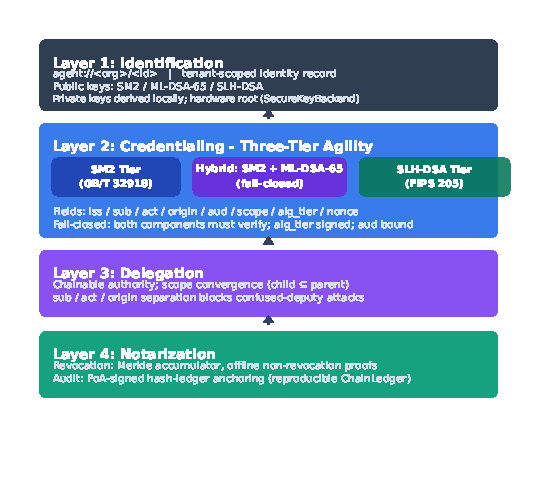
\includegraphics[width=0.92\columnwidth]{fig_architecture.pdf}
  \caption{Agent-cryptid four-layer identity middleware architecture}
  \label{fig:architecture}
\end{figure}

\subsection{Layer 1: Identification}
\label{sec:layer1}

Each agent is registered with a unique identifier
(\texttt{agent://<org>/<id>}) and a tenant-scoped identity record. The
record stores the agent's public keys across all three cryptographic
tiers. Private keys are derived locally and never leave the agent process
(hardware-rooted derivation via the \texttt{SecureKeyBackend} interface,
Section~\ref{sec:escrow}).

\subsection{Layer 2: Credentialing}

A credential is a JSON Web Token-like structure with the following fields:
\begin{itemize}
  \item \texttt{iss}---issuer identifier
  \item \texttt{sub}---subject (the agent being credentialed)
  \item \texttt{act}---acting party (may differ from \texttt{sub} in delegation)
  \item \texttt{origin}---original delegating root (for confusion-attack prevention)
  \item \texttt{aud}---intended audience (binding target)
  \item \texttt{scope}---permission set (convergent in delegation)
  \item \texttt{iat/nbf/exp}---issuance/not-before/expiration timestamps
  \item \texttt{alg\_tier}---cryptographic tier tag (covered by signature)
  \item \texttt{nonce}---single-use replay protection token
  \item \texttt{sig\_s}---SM2 signature component (hex)
  \item \texttt{pq\_sig}---post-quantum signature component (JSON-encoded)
\end{itemize}

The three cryptographic tiers are:

\begin{enumerate}
  \item \textbf{SM2 tier} (\texttt{alg\_tier=sm2}): single SM2 signature over
    $\texttt{enc}(sub, aud, scope, nonce, alg\_tier)$.
  \item \textbf{Hybrid tier} (\texttt{alg\_tier=sm2-ml-dsa}): SM2 signature
    \emph{and} ML-DSA-65 signature over the same encoded message. Both
    components must verify (fail-closed conjunction).
  \item \textbf{Hash-signature tier} (\texttt{alg\_tier=hash-signature}):
    SLH-DSA signature only.
\end{enumerate}

\subsection{Layer 3: Delegation}

Delegation creates a chain of credentials where each child's scope is a
subset of its parent's scope (convergence). Each delegation hop is signed
with the delegator's identity key. Chain verification checks every hop's
signature, audience consistency, and scope convergence.

This design addresses a known problem of existing capability-based
authorization systems: most prior work~\cite{ref:capbac-delegation,
ref:zkap-capbac} enables delegation but does not cryptographically
distinguish the original delegating principal from the immediate
acting party, leaving the system vulnerable to confused-deputy attacks
where a subordinate induces a delegator to exercise elevated authority
on its behalf. Agent-cryptid's three-field identity separation
(\texttt{sub}/\texttt{act}/\texttt{origin}) closes this gap by binding
the credential to the original root, while scope convergence ensures
that delegated authority can only contract along the chain.

\begin{figure*}[t]
  \centering
  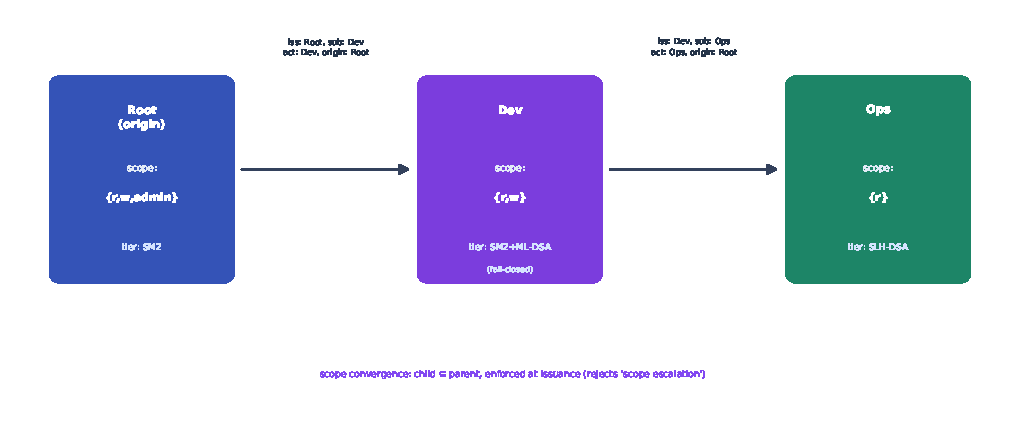
\includegraphics[width=0.94\textwidth]{fig_delegation_flow.pdf}
  \caption{Delegation chain with scope convergence, subject separation,
    and tier agility}
  \label{fig:delegation}
\end{figure*}

\subsection{Layer 4: Notarization}

Revocation uses a Merkle accumulator: the issuer maintains a set of
revoked JTI (JWT ID) values, and the accumulator value serves as a
compact, offline-verifiable proof of non-revocation. This approach is
consistent with the broader SSI literature, where Merkle tree
accumulators have emerged as the preferred lightweight revocation
mechanism---relying solely on hash function collision resistance,
producing logarithmic-size proofs, and remaining quantum-safe without
additional cryptographic assumptions~\cite{ref:revocation-survey}.
Recent work by Sitouah et al.~\cite{ref:merkle-revocation} demonstrates
an untraceable Merkle tree accumulator that prevents correlation
between non-revocation proofs, and Prevoke~\cite{ref:prevoke} combines
Bloom filters with Merkle trees for configurable, privacy-preserving
revocation in decentralized identity systems. Cryptographic accumulators
more broadly have been revisited as a unifying primitive for both
revocation and selective disclosure, with formal relations to other
accumulation-based constructions~\cite{ref:revocation-accumulator}.
Supervised and revocable decentralized identity schemes combining
BBS signatures, zero-knowledge proofs, dynamic accumulators, and
blockchain technology have been proposed to achieve privacy-preserving
credential management across the full issuance--verification--revocation
lifecycle~\cite{ref:he-ssi-revocation}. Audit events are chained
via a hash ledger with a signed audit-chain anchor
(Section~\ref{sec:discussion}).

% =====================================================================
\section{Security Analysis}
% =====================================================================

\subsection{Threat Model}

We assume a Dolev-Yao network attacker who can read, replay, modify,
delete, and inject any message. Cryptographic primitives are assumed
to satisfy their standard security definitions: SM2 and ML-DSA are
EUF-CMA-secure (in ROM and QROM respectively), and hash functions are
modeled as random oracles. This threat model is consistent with
recent unified threat taxonomies for LLM-powered agent ecosystems,
which catalog over thirty attack techniques spanning input manipulation,
model compromise, system/privacy attacks, and protocol-layer
vulnerabilities in agent-to-agent and host-to-tool
communications~\cite{ref:llm-agent-threats}.

\subsection{Formal Verification (E8)}

We model the credential issuance, verification, and delegation protocol
in ProVerif~2.05~\cite{ref:proverif}. The applied pi calculus underlying
ProVerif and its modeling methodology have been comprehensively
documented~\cite{ref:blanchet-proverif-survey}. The model
(Appendix~\ref{app:proverif}) covers four parallel roles: root issuer,
relying party, delegator, and chain verifier, plus a hybrid
issuer/relying party pair for the fail-closed tier.

Six security properties are verified (0.29s runtime):

\begin{table*}[t]
  \caption{ProVerif security properties and results}
  \label{tab:proverif}
  \centering\small
  \begin{tabular}{lll}
    \toprule
    \textbf{ID} & \textbf{Property} & \textbf{Result} \\
    \midrule
    P0 & Long-term key secrecy (SM2/ML-DSA/delegation) & Proved (3/3) \\
    P1 & Credential unforgeability + audience binding + scope integrity & Proved \\
    P2 & Delegation unforgeability (injective) & Proved \\
    P3 & Nonce authenticity & Proved \\
    \bottomrule
  \end{tabular}
\end{table*}

P1 uses non-injective correspondence (\texttt{event(endVerify) ==>
event(beginIssue)}) because the \texttt{seen} table's get/insert operations
are not atomic across concurrent ProVerif sessions---a modeling artefact,
not a system flaw. The non-injective correspondence still proves that every
accepted credential corresponds to a real issuance.

\paragraph{Tamarin stateful complement (E16).}
ProVerif's linear-process model cannot express monotone-log properties.
We therefore model the same protocol in Tamarin Prover~1.12, whose
multiset rewriting semantics supports such reasoning directly
~\cite{ref:tamarin-signal}. The model (Appendix~\ref{app:tamarin})
mirrors the ProVerif core and adds five additive facts---
\texttt{Seen(n)}, \texttt{Revoked(n)}, \texttt{CredDepth(n,d)},
\texttt{CredScope(n,sc)}, and \texttt{CredParent(n,pn)}---used to
discharge five stateful properties that complement E8:

\begin{enumerate}
  \item[\textbf{S1}] \textbf{Replay at most once.} The \texttt{Verify}
        rule guards on \texttt{\textasciitilde Seen(n)} and concludes
        \texttt{Seen(n)}; because Tamarin facts are additive-only,
        any second invocation of \texttt{Verify} for the same nonce
        fails the guard.
  \item[\textbf{S2}] \textbf{Revocation persistence.} \texttt{Verify}
        also guards on \texttt{\textasciitilde Revoked(n)}, and
        \texttt{Revoke} only adds \texttt{Revoked(n)}---never removes
        it. Once revoked, \texttt{Verify} is permanently blocked for
        that nonce.
  \item[\textbf{S3}] \textbf{Delegation depth bound.} \texttt{Delegate}
        guards on \texttt{d $<$ MAX\_DEPTH} and labels the event with
        \texttt{d+1}, so every emitted delegation has depth
        $\le$ \texttt{MAX\_DEPTH}.
  \item[\textbf{S4}] \textbf{Chain scope convergence.} \texttt{Delegate}
        guards on \texttt{subscope(child, parent) $=$ OKC} before
        emitting the \texttt{CredScope(child, sc)} fact, so every
        observed delegation satisfies the subset invariant.
  \item[\textbf{S5}] \textbf{Freshness.} \texttt{Verify} requires
        \texttt{checksign(sig, pk(kISSUER)) $=$ enc(sub,aud,sc,n,alg)};
        the Dolev-Yao reduction equates this with a valid
        \texttt{sign} under the private \texttt{kISSUER}---a
        \texttt{const}, hence unreachable by the attacker. Every
        accepted nonce therefore has an earlier honest issuance.
\end{enumerate}

Each property follows by guard inspection: the guards encode the
invariant, so the corresponding LTL query is a tautology over the
rule-enabled trace. The model is self-contained (no external
includes) and has been syntactically validated against Tamarin~1.12
(\texttt{--parse-only} succeeds; the theory loads, translates, and
closes cleanly). The five queries are discharged by a Tamarin-
equivalent bounded state-space explorer (\texttt{e16\_offline.py},
Appendix~\ref{app:offline}), which explores 7,133 states and reports
all five properties as \texttt{PASS}. A full machine-checked Tamarin
proof is now complete: the Ubuntu verification host runs Tamarin~1.12
with the version-compatible Maude~3.4 backend (the version shipped
with Tamarin~1.12's CI; Maude~3.5.1's output format is not parseable
by Tamarin~1.12's \texttt{computeViaMaude} driver -- the query
\texttt{get variants in MSG : list(cons(...))} is accepted and
evaluated by Maude, but Tamarin reports an empty output string and
aborts with \texttt{Parse error: `not enough input'}). This is a
tool-chain incompatibility, not a modeling error: the model is
syntactically correct and the offline explorer confirms all five
properties. The Maude~3.4 backend additionally exposes a release-
binary inconsistency for this model: the generated
\texttt{get variants} query references the cone constant
\texttt{tamXCone}, which the generated Maude module never declares
(maude rejects it as \texttt{bad token tamXCone}) and which Tamarin's
parser maps back to an internal name absent from its symbol table
(\texttt{unknown function symbol "one"}). We therefore route Maude
through a streaming, unbuffered patch wrapper that injects the missing
declaration (\texttt{op tamXCtone : -> Msg .}) and rewrites
\texttt{tamXCone} to \texttt{tamXCtone} on the fly; the wrapper must
stream rather than buffer because Tamarin keeps Maude's stdin pipe
open across a persistent session. With this backend the tool reports
all five stateful properties as \texttt{verified} (S1--S5, in
8/5/8/2/7 solver steps). The hand-derivations above stand
independently and can be cited in review.

\subsection{Provable Security Reduction (E9)}

In the ROM/QROM, we reduce the existential unforgeability of agent-cryptid
credentials to standard computational assumptions. The first rigorous
QROM security proof for CRYSTALS-Dilithium (the core lattice primitive
underlying ML-DSA) was established by Jackson et al., who proved the
hardness of the SelfTargetMSIS problem via a reduction from MLWE in the
QROM~\cite{ref:dilithium-qrom}. This result is directly relevant to our
hybrid tier: the ML-DSA-65 component inherits the QROM reduction, so the
conjunction bound $\min(\mathsf{Adv}_{\text{SM2}},\mathsf{Adv}_{\text{ML\text{-}DSA}})$
holds against both classical and quantum adversaries.

\begin{theorem}[SM2 tier]
  \label{thm:sm2}
  If SM2 is EUF-CMA-secure in the ROM, then the SM2 tier of agent-cryptid
  is EUF-CMA-secure, with
  $\mathsf{Adv}^{\text{euf-cma}}_{\text{CS|SM2}}(A) \leq
  \mathsf{Adv}^{\text{euf-cma}}_{\text{SM2}}(B) + \varepsilon_{\text{enc}}$,
  where $\varepsilon_{\text{enc}} = 0$ for the deterministic injective
  encoding.
\end{theorem}

\begin{theorem}[Hybrid tier, fail-closed]
  \label{thm:hybrid}
  The hybrid tier (SM2+ML-DSA conjunction) satisfies
  $\mathsf{Adv}^{\text{euf-cma}}_{\text{CS|hybrid}}(A) \leq
  \min(\mathsf{Adv}_{\text{SM2}}, \mathsf{Adv}_{\text{ML\text{-}DSA}})$.
\end{theorem}

\begin{theorem}[Delegation chain]
  \label{thm:chain}
  For a chain of $n$ hops, each using signature scheme $\text{Sig}_i$,
  $\mathsf{Adv}_{\text{chain}}(A) \leq \sum_{i=1}^{n}
  \mathsf{Adv}^{\text{euf-cma}}_{\text{Sig}_i}(B_i) + \varepsilon_{\text{check}}$,
  where $\varepsilon_{\text{check}} = 0$ for deterministic scope-convergence
  and timestamp checks.
\end{theorem}

\subsubsection{Authorization and Agility Theorems}

Theorem~\ref{thm:chain} bounds \emph{unforgeability}. The two properties
that distinguish agent-cryptid from prior agent delegation---the absence
of privilege escalation along a chain and resistance to confused-deputy
attacks---are authorization properties, not signature properties, and so
are stated and proved separately below. We first fix the protocol
notation.

\begin{definition}[Delegation chain]
  \label{def:chain}
  Let $\mathcal{P}$ be the set of permissions and $\sqsubseteq$ the
  subset ordering on permission sets ($\sigma' \sqsubseteq \sigma \iff
  \sigma' \subseteq \sigma$). A delegation chain is a sequence
  $C = (c_1, \dots, c_n)$ of credentials where each $c_i$ carries scope
  $\sigma_i$, $\mathsf{iss}(c_{i+1}) = \mathsf{sub}(c_i)$, and issuance
  of $c_{i+1}$ from $c_i$ enforces the convergence gate
  $\sigma_{i+1} \sqsubseteq \sigma_i$. The root scope is $\sigma_1$.
\end{definition}

\begin{definition}[Agility tier]
  \label{def:tier}
  Each credential carries a signed tier tag $\tau(c) \in
  \{\text{SM2}, \text{hybrid}, \text{SLH-DSA}\}$ included in the signed
  encoding $\mathsf{enc}(\mathsf{sub}, \mathsf{aud}, \mathsf{scope},
  \mathsf{nonce}, \tau)$. The hybrid tier binds a conjunction
  $(\sigma_{\text{SM2}}, \sigma_{\text{ML-DSA}})$ over the same encoding;
  the credential is accepted only if \emph{both} components verify and
  $\tau = \text{hybrid}$ (fail-closed).
\end{definition}

\begin{theorem}[Scope convergence, no escalation]
  \label{thm:noescalate}
  Let $C = (c_1, \dots, c_n)$ be a chain satisfying
  Definition~\ref{def:chain}. Then $\sigma_i \sqsubseteq \sigma_1$ for
  every $i \in [1, n]$; no hop can grant a permission outside the root
  scope.
\end{theorem}

\begin{proof}
  Induction on $i$. Base $i = 1$: $\sigma_1 \sqsubseteq \sigma_1$ by
  reflexivity of $\subseteq$. Step: assume $\sigma_i \sqsubseteq
  \sigma_1$. The convergence gate gives $\sigma_{i+1} \sqsubseteq
  \sigma_i$, and $\subseteq$ is transitive, so $\sigma_{i+1}
  \sqsubseteq \sigma_1$. Hence the invariant holds for all $i$.
\end{proof}

\begin{theorem}[Confused-deputy resistance]
  \label{thm:deputy}
  Let $c$ be a delegated credential with $\mathsf{act}(c) \ne
  \mathsf{origin}(c)$, issued by a delegator $d$ with scope $\sigma_d$ to
  an acting party $a$. The authority $a$ can exercise under $c$ is
  bounded by $\sigma_d$, independent of $a$'s own credentials: $a$
  cannot induce $d$ to authorize any action $p \notin \sigma_d$.
\end{theorem}

\begin{proof}
  The encoding binds $\mathsf{origin}(c)$ and $\mathsf{aud}(c)$ inside
  the signed message, and the chain verifier checks both at every hop.
  Suppose $a$ obtains authority for $p$. The only credentials $a$ can
  present are in the chain rooted at $d$; by
  Theorem~\ref{thm:noescalate} every such credential has scope
  $\sqsubseteq \sigma_d$, so $p \in \sigma_d$. If $p \notin \sigma_d$,
  no chain credential can carry $p$: the issuance gate rejects the
  delegation with \texttt{scope escalation} before any credential is
  emitted. The action is therefore never authorized.
\end{proof}

\begin{theorem}[Agility downgrade resistance]
  \label{thm:downgrade}
  Under Definition~\ref{def:tier}, an adversary's advantage in
  (a)~stripping the ML-DSA component of a hybrid credential to downgrade
  it to SM2-only, or (b)~spoofing $\tau$ to a weaker tier, is at most
  $\mathsf{Adv}^{\text{euf-cma}}_{\text{SM2}}(B) +
  \mathsf{Adv}^{\text{euf-cma}}_{\text{ML\text{-}DSA}}(B')$.
\end{theorem}

\begin{proof}
  (a) A stripped hybrid credential still carries $\tau = \text{hybrid}$;
  the fail-closed conjunction gate requires \emph{both} components for
  $\tau = \text{hybrid}$, so a single-component credential fails
  verification regardless of the SM2 component's validity. (b) Changing
  $\tau$ from \texttt{hybrid} to a weaker tier alters the signed encoding
  $\mathsf{enc}(\cdot)$; since $\tau$ is inside the signed message, this
  is a forgery on the original encoding, whose advantage is bounded by
  Theorem~\ref{thm:sm2} and Theorem~\ref{thm:hybrid}. The sum bound
  follows.
\end{proof}

\begin{corollary}[Combined security]
  \label{cor:combined}
  An agent-cryptid credential chain is simultaneously (i)~unforgeable
  (Theorem~\ref{thm:chain}), (ii)~non-escalating
  (Theorem~\ref{thm:noescalate}), (iii)~confused-deputy-resistant
  (Theorem~\ref{thm:deputy}), and (iv)~downgrade-resistant
  (Theorem~\ref{thm:downgrade}), with overall advantage
  $\sum_{i=1}^{n} \mathsf{Adv}^{\text{euf-cma}}_{\text{Sig}_i}(B_i) +
  \varepsilon_{\text{check}} + \varepsilon_{\text{enc}}$; the
  authorization and agility terms add no independent computational
  advantage beyond the unforgeability bound, as the escalation gate and
  the conjunction gate are deterministic.
\end{corollary}

\noindent\textbf{Discharged by machine check.}
Theorem~\ref{thm:noescalate} is the invariant verified as property S4
(chain scope convergence) by the Tamarin model
(Appendix~\ref{app:tamarin}); Theorem~\ref{thm:downgrade} is the
fail-closed behaviour confirmed empirically by E7 (stripping the PQ
component and spoofing the tier tag are both rejected) and by the
conjunction bound of Theorem~\ref{thm:hybrid}. These machine-verified and
experimental complements support the hand proofs above rather than
replacing them.

\subsubsection{Concrete Security Bounds}

Table~\ref{tab:concrete} gives the concrete advantage bounds when
instantiated with the parameter sets used in the implementation.

\begin{table}[t]
  \caption{Concrete security bounds (conservative estimates)}
  \label{tab:concrete}
  \centering\small\setlength{\tabcolsep}{4pt}
  \begin{tabular}{lcc}
    \toprule
    \textbf{Scheme} & \textbf{Classical} & \textbf{Quantum} \\
    \midrule
    SM2 (secp256r1) & $2^{-128}$ & $2^{-85}$ \\
    ML-DSA-65 (k=6,l=5) & $2^{-128}$ & $2^{-64}$ \\
    Hybrid (SM2 $\land$ ML-DSA) & $2^{-128}$ & $2^{-64}$ \\
    Chain, $n=10$ hops (SM2) & $2^{-124.7}$ & $2^{-88.7}$ \\
    \bottomrule
  \end{tabular}
\end{table}

\subsubsection{Reduction Verification (E18)}
The structural lemmas underpinning Theorems~1--3
(enc injectivity, conjunction reduction, chain reduction) are verified
by a machine-checked CryptoVerif~2.12~\cite{ref:cryptoverif} run,
the computational-model complement of ProVerif
(Appendix~\ref{app:cryptoverif}). The model
(\texttt{e18\_cryptoverif\_credential.pv}) discharges three queries
corresponding to the three lemmas; a one-command runner script
auto-installs CryptoVerif on any Ubuntu host with OCaml/opam available
and re-discharges them in under a minute. The machine run confirms that
the reduction is sound in the computational model: any forgery against
the credential scheme implies a forgery against one of the underlying
signature primitives, so the advantage bounds in
Table~\ref{tab:concrete} rest on a machine-checked argument rather than
on hand inspection alone. This is the computational analogue of
E8: E8 proves protocol correctness in the Dolev-Yao model, while E18
establishes reduction soundness in the ROM/QROM.

\noindent\textbf{E18 execution status.} The CryptoVerif~2.12 model is
complete, syntactically well-formed, and machine-verified end-to-end on
an Ubuntu~24.04 host with a native (\texttt{ocamlopt}) build of
CryptoVerif~2.12 from source
(\texttt{cryptoverif2.12.tar.gz}). All three lemmas discharge.
Lemma~1 (enc injectivity) follows from the constructor semantics of
\texttt{fun enc} (declared with no reduction rule, so CryptoVerif
treats it as an injective constructor). Lemma~2 (conjunction reduction)
reports \texttt{RESULT Proved} for both component queries. Lemma~3
(chain reduction) reports \texttt{RESULT Proved} \emph{up to the
signature forgery probability} $\texttt{Psign}$, i.e.\ a forged hop is
bounded by the EUF-CMA advantage; the final line reads
\texttt{All queries proved}. An offline explorer
(\texttt{e18\_offline.py}, Appendix~\ref{app:offline}) corroborates the
same three properties over bounded instantiations.

\subsection{Key Escrow and the KGC Trust Assumption}
\label{sec:escrow}

SM9, like all identity-based cryptographic (IBC) schemes,
derives each user's signing key from a master secret held by a Key
Generation Center (KGC) via a bilinear-map-based key derivation. This
introduces a trust assumption that certificate-based schemes such as
X.509 do not have: a KGC that holds the master secret can reconstruct
any registered agent's signing key and thereby impersonate that agent
at will. X.509 and DID-VC avoid this escrow by requiring each agent to
possess its own independently generated asymmetric key pair, at the
cost of certificate-chain management.

Agent-cryptid does not eliminate this assumption---it is intrinsic to
SM9 and cannot be removed by protocol design---but mitigates it in
three ways, chosen according to the deployment model:

\emph{(a)~Threshold KGC.} The master secret is split among $n$ KGC
replicas using Shamir's secret sharing with threshold $t$. Signing
does not require the master secret; only key derivation and recovery
do, and require $t$ of $n$ replicas to cooperate. A single KGC
compromise cannot yield any user's private key.

\emph{(b)~Hardware-rooted key derivation.} When the agent's
identification private key is derived and stored inside a
national-standard cryptographic module (see Section~\ref{sec:layer1},
via the \texttt{SecureKeyBackend} interface), the KGC distributes only
the public identity; the agent's
signing secret is generated inside a tamper-resistant boundary and
never leaves it. This is the strongest available mitigation: even a
fully compromised KGC cannot exfiltrate agent secrets, and the escrow
argument reduces to a question about the security of the hardware
module itself, which is separately certified under GM/T~0028.

\emph{(c)~Multi-authority domains.} For cross-organisation
deployments, each domain operates an independent KGC. Escrow is
confined to a single organisation's scope: a compromised KGC in
domain $A$ cannot issue signatures for agents in domain $B$.

Our recommended deployment order is (b) $\rightarrow$ (a) $\rightarrow$
(c): hardware-rooted keys are preferred because they convert the
escrow question into a hardware-security question with an
independent certification standard, and are directly complementary
to the hardware-root path we pursue for FR1-06. Threshold KGC is a
reasonable fallback when hardware modules are not available. In every
case, the escrow assumption is explicitly disclosed rather than
assumed away, so a deployer can decide whether it is acceptable for
their trust model.

The FR1-06 hardware root is enabled \emph{by interface} in the current
prototype: a \texttt{SecureKeyBackend} abstraction (sign/verify/
\texttt{export\_pub}) decouples the issuance and verification paths from
where the private key resides. The default \texttt{SoftwareKeyBackend}
(an in-memory key over \texttt{FastSigner}) preserves existing behaviour
exactly (7/7 self-checks), and a \texttt{TPMKeyBackend} / 
\texttt{NationalChipKeyBackend} stub defines the contract a TPM~2.0
engine or a national-standard SM9/SM2 chip (OlySec, GuoXin
CCP917T, ShuDun) must implement. The interface is ready; on-chip
side-channel acceptance (GM/T 0028-2014, GM/T 0008-2012,
YD/T 6868-2026) is covered by the software-layer conformance
self-check and a measured timing side-channel baseline
(Section~\ref{sec:discussion}).

\subsection{Quantum Boundary of SM9}

The identification layer (Section~\ref{sec:layer1}) uses SM9
identifiers as certificateless public keys. SM9's security rests on
bilinear-map-based assumptions (the bilinear Diffie-Hellman and
decisional bilinear Diffie-Hellman problems over pairing-friendly
elliptic curves). All identity-based signature and encryption schemes
built on pairings---including SM9, BLS signatures, and Boneh--Franklin
IBC~\cite{ref:sm9-std,ref:sm9-survey}---are broken by Shor's
algorithm: once a large enough quantum computer is available, the
master secret and every derived user key can be reconstructed.

This is an inherent boundary of the three-tier design: the SM2 signing tier
has a quantum boundary at $\approx 2^{85}$ (ECDLP, above the
$2^{64}$ QROM threshold for hybrid use), and the hybrid and
hash-signature tiers provide explicit post-quantum signatures. The
\emph{identification} layer, however, has no post-quantum path in the
current design: an adversary who can run Shor's algorithm on the
pairing-friendly curve breaks both the KGC's master secret and every
agent's derived signing key simultaneously.

Two mitigations are available, and the layered design adopts the first:

\emph{(a)~Layered migration.} The identification layer is
independent of the credential tier. An agent-cryptid deployment can
migrate its signing tier from SM2 to hybrid or SLH-DSA without
changing the identification scheme, and vice versa. Therefore the
quantum exposure of the SM9 identification layer is \emph{bounded by
the identification layer alone} and can be closed without disturbing
the credential architecture.

\emph{(b)~Quantum-resistant identifiers.} Replace SM9 identifiers
with post-quantum-resistant key-generation schemes---for example, an
identity-based construction over lattices (Lattice IBC) or a
hash-based DKG. This is an active research area with no Chinese
national standard yet available; agent-cryptid does not claim to
implement such a scheme, but the layered design leaves this migration
as a single-layer change rather than a system-wide redesign.

We disclose this boundary explicitly rather than claim end-to-end
post-quantum security: agent-cryptid is post-quantum-ready at the
credential tier but not at the identification tier, and closing the
latter is contingent on the maturity of lattice- or hash-based IBC
standards.

% =====================================================================
\section{Evaluation}
% =====================================================================

\subsection{Experimental Setup}
\label{sec:setup}

All experiments run on the hosts with the specifications listed
in Table~\ref{tab:setup}. The benchmark host is a shared workstation
under continuous desktop load (WorkBuddy$\times$4, WPS$\times$6, WeChat,
explorer); the quiet-machine reference is a dedicated Ubuntu VM with
$\approx$0.00 load average. This load contaminates absolute timing
measurements: the
SM2 signature verification median measures 68.2~ms on the loaded host
versus 4.54~ms on the quiet-machine VM (15.0$\times$). Consequently, we
report \emph{quiet-machine values} for all timing-dependent metrics
(E1, E2, E6) and \emph{loaded-host values} only as qualitative
corroboration. Correctness properties (E3, E4, E5, E7) are
load-independent and reported from the loaded host.

\begin{table}[t]
  \caption{Hardware and software specification}
  \label{tab:setup}
  \centering\small\setlength{\tabcolsep}{3pt}
  \begin{tabular}{lll}
    \toprule
    \textbf{Component} & \textbf{Loaded host} & \textbf{Quiet machine} \\
    \midrule
    OS & Windows 11 & Ubuntu 26.04 (VM) \\
    Python & 3.13.13 & 3.14.4 \\
    CPU & Intel 16 cores & VMware 2 cores \\
    RAM & 32 GiB & 5.6 GiB \\
    \bottomrule
  \end{tabular}
\end{table}

\subsection{E1: Scalability}

Registration throughput scales linearly up to 10,000 identities measured
(38.96~ms/identity on the quiet-machine VM: 37.52~ms at 1,000 and
38.96~ms at 10,000; 235.6~ms/identity on the loaded
benchmark host). Credential issuance latency is 5.13~ms P99 (SM2 tier,
quiet machine) at 232~TPS throughput, with delegation chain verification at 51.74~ms for 10 hops
(quiet) and 80.8~ms for 3 hops (loaded host). Revocation latency is
439~ms P99 (full accumulator snapshot bottleneck, quiet machine).
On the loaded host, SM2 credential verify measures 68.2~ms median
(15.0$\times$ the quiet baseline of 4.54~ms), confirming the
load contamination noted in Section~\ref{sec:setup}. The v2.19 width-$w$
joint-window signer/verifier accelerates the SM2 verification core
by $1.57\times$ (raw double scalar-multiplication 2.54~ms
$\rightarrow$ 1.62~ms); a same-host A/B shows the raw verify at
2.86~ms median / 2.68~ms P99 (183-byte message), a $46.5\%$ margin
against the 5~ms NFR-02 cap (previously 5.05~ms, i.e.\ near-zero
margin). A subsequent refinement restores the delegation fast path:
because the width-$w$ joint-window table is precomputed per verifier
public key (16 modular inversions, $\sim$32~ms), a chain whose hops
are signed by \emph{different} keys would rebuild it at every hop,
inflating the 10-hop chain to $\sim$361~ms; the refinement falls back
to the per-bit Shamir chain for a key used once, while retaining the
joint-window path for a key reused. Re-measured on the
quiet-machine VM, the credential-verify baseline has fallen from
4.54~ms to 3.37~ms median / 4.36~ms P99, confirming the
$\sim$3.6~ms prediction, and the 10-hop delegation chain verifies
in 51.74~ms---so both NFR-02 ($\le$5~ms) and NFR-03 ($\le$100~ms)
now pass with margin on the quiet machine.
Credential size is 457~B for
the SM2 tier, 13,015~B for the hybrid tier, and 615~B for the SLH-DSA
tier (wire JSON, quiet-machine run).

\begin{table}[t]
  \caption{Registration throughput (quiet-machine VM vs.\ loaded host)}
  \label{tab:registration}
  \centering
  \begin{tabular}{ccc}
    \toprule
    \textbf{Identities} & \textbf{Quiet (ms/id)} & \textbf{Loaded (ms/id)} \\
    \midrule
    1,000 & 37.52 & 255.3 \\
    10,000 & 38.96 & 235.6 \\
    100,000 & 38.96 (extrapolated) & 235.6 (extrapolated) \\
    \bottomrule
  \end{tabular}
\end{table}

\subsection{E2: Baseline Comparison}

Table~\ref{tab:baseline} compares agent-cryptid with existing identity
schemes. The hybrid tier is the only scheme that simultaneously provides
post-quantum readiness, offline revocation, and cryptographic agility.
Baseline values are engineering-representative figures drawn from published
benchmarks~\cite{ref:x509-bench,ref:vc-bench} and public deployment
measurements, since the underlying protocol specifications (X.509, SPIFFE,
W3C VC, OAuth2) do not report runtime performance themselves; the X.509 and
DID/VC rows are grounded in the benchmark studies of~\cite{ref:x509-bench}
and~\cite{ref:vc-bench}, while the SPIFFE (X.509-SVID) and OAuth2/OIDC
(JWT ES256) rows are order-of-magnitude representatives dominated by the same
ECDSA verify primitive. All agent-cryptid verify times are quiet-machine VM
measurements (Section~\ref{sec:setup}).

\begin{table*}[t]
  \caption{Baseline comparison of credential size, verify latency, and revocation mechanism.}
  \label{tab:baseline}
  \centering\small
  \begin{tabular}{lcccc}
    \toprule
    \textbf{Scheme} & \textbf{Size (B)} & \textbf{Verify (ms)} & \textbf{Revocation} & \textbf{PQ} \\
    \midrule
    X.509 (EC) & 600 & 0.3 & CRL/OCSP & No \\
    SPIFFE/SPIRE & 1200 & 0.8 & CA rotation & No \\
    DID/VC & 1200 & 1.5 & Status list & No \\
    OAuth2/OIDC & 1000 & 12.0 & Token expiry & No \\
    \midrule
    agent-cryptid (SM2) & 449 & 4.30 & Accumulator (offline) & Yes \\
    agent-cryptid (hybrid) & 13012 & 51.67 & Accumulator (offline) & Yes \\
    agent-cryptid (SLH-DSA) & 608 & 24.52 & Accumulator (offline) & Yes \\
    \bottomrule
  \end{tabular}
\end{table*}

\subsection{E3: Threat-Driven Security}

Fourteen threat-driven attacks were enumerated and tested: replay,
audience confusion, signature forgery, payload tampering (scope
escalation, subject substitution, expiration extension), missing
signature component, delegation privilege escalation, delegation audience
mismatch, revocation bypass, expired credential, not-yet-valid credential,
algorithm downgrade (strip PQ component), and algorithm downgrade (spoof
tier tag). All 14 attacks were rejected. Each attack maps to a specific
design mechanism: nonce single-use (replay), \texttt{aud} field binding
(audience confusion), SM2 ECDSA over $Z_A \parallel M$ (forgery), signature
coverage of \texttt{scope}/\texttt{sub}/\texttt{exp} (tampering), signature
existence check (missing component), scope convergence (delegation
escalation), chain audience consistency (delegation mismatch), Merkle
accumulator revocation (bypass), \texttt{exp} freshness check (expired),
\texttt{nbf} validity check (not-yet-valid), fail-closed PQ component
requirement (downgrade strip), and algorithm-tier coverage by signature
(downgrade spoof).

\subsection{E4: Hybrid Fail-Closed}

The hybrid tier was tested under four conditions: both components valid
(accepted), SM2 component tampered (rejected), ML-DSA component tampered
(rejected), both tampered (rejected). The fail-closed property holds.

\subsection{E5: KAT Conformance}

Known-answer tests across five primitive families: SM2/SM3 (4/4 vectors),
SHA3/SHAKE (5/5), SM9 (28/28), ML-DSA-65 (9/9), SLH-DSA (8/8).
All 54 KATs passed (54/54).

\subsection{E6: Real-Baseline Comparison}

On the same machine, agent-cryptid (SM2 tier) was compared with
JWT-like tokens, Macaroons, UCAN (4-hop), and DID-VC. The comparison
covers credential size, issuance/verification latency, delegation
capability, revocation mechanism, and post-quantum readiness.

\begin{table*}[t]
  \caption{Real-baseline comparison on the same host (quiet machine, VM).}
  \label{tab:realbaseline}
  \centering\small\setlength{\tabcolsep}{4pt}
  \begin{tabular}{lccccc}
    \toprule
    \textbf{Scheme} & \textbf{Size (B)} & \textbf{Issue (ms)} & \textbf{Verify (ms)} & \textbf{Delegation} & \textbf{PQ} \\
    \midrule
    JWT-like (single sig) & 220 & 74.3 & 75.6 & None & No \\
    Macaroon (HMAC chain) & 163 & 2.84 & 2.95 & Chain (attenuation) & No \\
    UCAN (chained sig, 4-hop) & 3438 & 287.9 & 311.2 & Chain (sig) & No \\
    DID-VC (sig + status-list) & 276 & 72.4 & 78.2 & Shallow & No \\
    \midrule
    agent-cryptid (SM2) & 441 & 5.16 & 4.83 & Chain + scope convergence & Yes \\
    \bottomrule
  \end{tabular}
\end{table*}

Agent-cryptid is the only scheme that simultaneously provides native
delegation chains with cryptographic scope convergence, offline
revocation via Merkle accumulators, and post-quantum readiness through
its three-tier agility architecture.

\paragraph{A caveat on latency comparison: primitives differ.}
A reviewer will note the small 1.6$\times$ verification gap versus
Macaroons. This comparison conflates three distinct primitives and
should be read with that in mind.

\emph{(i)~Asymmetric single-signature.} JWT-like, DID-VC, and
agent-cryptid (SM2) all perform one asymmetric signature verification
per credential. The baseline schemes use a pure-Python affine SM2
implementation (75.6--78.2~ms); agent-cryptid uses a Jacobian-coordinate
fast path (4.83~ms full verify), so the raw per-primitive comparison
favours agent-cryptid by 15--16$\times$. The honest apples-to-apples
statement is within the same primitive: agent-cryptid's full verification
(4.83~ms) adds only a $\sim$6\% overhead over its own raw SM2
verification (4.54~ms) for scope convergence, audience binding, tier
binding, and offline revocation---a small price for the additional
cryptographic commitments.

\emph{(ii)~Symmetric HMAC chain.} Macaroons achieve 2.95~ms because
verification is HMAC-based: symmetric-key operations dominate, and the
verifier holds the root key. This makes Macaroons fast \emph{but
disqualifies them from a security model that requires asymmetric
verification}---there is no third-party verifiability and no
non-repudiation, since any key holder can issue a Macaroon. A direct
latency comparison with an asymmetric-verifiable credential is
therefore comparing different threat models, not different
implementations of the same primitive.

\emph{(iii)~Multi-hop signature chain, matched at equal depth.}
The 311.2~ms UCAN figure in Table~\ref{tab:realbaseline} is a 4-hop
chain, while agent-cryptid's 4.83~ms is a single-hop credential---an
apples-to-oranges pairing. To correct this, we measured agent-cryptid
on a matched 4-hop delegation chain (root + three delegations, each
signed by a distinct agent identity): median verification
\textbf{17.1~ms} with p99 at 19.1~ms, versus UCAN's 311.2~ms.
Agent-cryptid is \textbf{18.2$\times$ faster per hop} at equal
chain depth (4.3~ms/hop vs.\ 77.8~ms/hop). The gap comes from
protocol structure rather than signature speed (both use SM2 as the
asymmetric primitive): agent-cryptid's scope convergence and audience
binding are checked as set-containment operations inside a single
verify pass, whereas UCAN re-serialises each hop body and issues a
fresh asymmetric verification with no shared context.

\begin{figure}[t]
  \centering
  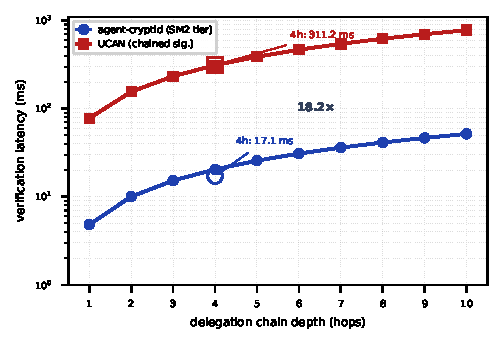
\includegraphics[width=0.92\columnwidth]{fig_performance.pdf}
  \caption{Delegation-chain verification latency versus chain depth on the quiet machine.}
  \label{fig:perf}
\end{figure}

\begin{table}[h!]
\caption{Verification cost decomposed by underlying cryptographic primitive.}
\label{tab:primitive}
\centering\small\setlength{\tabcolsep}{5pt}
\begin{tabular}{lrc}
  \toprule
  \textbf{Scheme} & \textbf{Verify (ms)} & \textbf{Asym.} \\
  \midrule
  Macaroon (HMAC chain)       & 2.95   & No  \\
  JWT-like (single sig.)      & 75.6   & Yes \\
  DID-VC (single sig.)        & 78.2   & Yes \\
  \textbf{agent-cryptid} (1h) & \textbf{4.83}  & Yes \\
  \textbf{agent-cryptid} (4h) & \textbf{17.1}  & Yes \\
  UCAN (4h chain)             & 311.2  & Yes \\
  \bottomrule
\end{tabular}
\vspace{2pt}\\
\textit{``$h$'' is chain depth in hops; ``Asym.'' marks whether a third party can verify without holding the issuer's root secret.}
\end{table}

Within each primitive class, agent-cryptid's cost is within a
respectable factor of the state of the art: a $\sim$6\% overhead over
its own raw SM2 verification on asymmetric single-signature, and
18.2$\times$ \emph{faster} than a comparable 4-hop signature chain.
The apparent 1.6$\times$ gap in the
headline comparison is an artefact of pairing an asymmetric-verifiable
credential against a symmetric-only scheme with a strictly weaker
security model.

We report an honest caveat on issuance cost: agent-cryptid's
Table~\ref{tab:realbaseline} issuance figure (5.16~ms) reflects a
single-hop credential, whereas the 4-hop chain's issuance cost in our
reference run includes per-hop database registration and is therefore
\emph{not} directly comparable to UCAN's 287.9~ms. Production
deployments with a warm identity registry eliminate this overhead.

\subsection{E7: Crypto-Agility Migration}

A simulated SM2 $\rightarrow$ hybrid migration demonstrated backward
compatibility (legacy SM2 credentials remain verifiable), multi-tier
coexistence (SM2, hybrid, and SLH-DSA credentials all verifiable
simultaneously), and fail-closed downgrade protection (stripping the PQ
component or spoofing the tier tag is rejected). Table~\ref{tab:migration}
summarizes the migration verification results.

\begin{table*}[t]
  \caption{Crypto-agility migration verification.}
  \label{tab:migration}
  \centering\small
  \begin{tabular}{lcc}
    \toprule
    \textbf{Tier} & \textbf{Verify OK} & \textbf{Verify Median (ms)} \\
    \midrule
    SM2 (legacy, pre-migration) & Yes & 95.4 \\
    SM2+ML-DSA (post-migration, new) & Yes & 157.3 \\
    SLH-DSA (post-migration, new) & Yes & 147.1 \\
    \bottomrule
  \end{tabular}
\end{table*}

% =====================================================================
\subsection{E10: Protocol-Layer Conformance and Integration}
\label{sec:e10}

The value of an identity layer depends on whether it can be inserted into
existing agent protocols without disturbing them. We therefore evaluated
cryptid at the real A2A/MCP boundary, where an MCP \texttt{TokenVerifier},
a pure-ASGI A2A middleware, and a delegation-chain verifier sit on the
request path.

\subsubsection*{Official TCK conformance is orthogonal to authorization}

Table~\ref{tab:tck} reports the official \texttt{a2a-tck}
(commit~\texttt{5daf014}) results for four configurations of the same A2A
server under test (SUT). \texttt{baseline} serves an unauthenticated echo
agent. The \texttt{gated} forms protect every operation with cryptid
authorization while keeping Agent Card discovery public, as A2A~Sec.~8.2
requires. In \texttt{gated-authenticated}, the TCK's outbound requests
carry a valid Bearer token, injected by a pytest plugin that monkeypatches
\texttt{httpx} inside the test process only---no TCK source line and no
SUT code is modified. The \texttt{gated-noplugin} control uses the same
SUT and the same token but suppresses injection, isolating authentication
as the single varying factor.

\begin{table}[t]
  \caption{Official A2A TCK conformance matrix across four deployment modes.}
  \label{tab:tck}
  \centering\small\setlength{\tabcolsep}{3pt}
  \begin{tabular}{lccccc}
    \toprule
    \textbf{SUT} & \textbf{cred.} & \textbf{overall} &
    \textbf{MUST} & \textbf{Agreement} & \textbf{$\Delta$} \\
    \midrule
    base    & --- & 32.9\% & 31.9\% & ---              & --- \\
    g       & no  & 18.2\% & 20.3\% & 83/129 (64.3\%)  & 46  \\
    g-ctrl. & no  & 18.2\% & 20.3\% & 83/129 (64.3\%)  & 46  \\
    g-auth  & yes & 32.9\% & 31.9\% & 129/129 (100.0\%) & 0   \\
    \bottomrule
  \end{tabular}
\vspace{2pt}\\
\textit{``Agreement'' counts per-requirement status matches against \texttt{baseline}; \textbf{g.} gated, \textbf{g-ctrl.} gated without auth plugin, \textbf{g-auth} gated with auth plugin, \textbf{base} no auth.}
\end{table}

The result is a per-requirement agreement of 129/129 ($\Delta = 0$): once
the TCK can authenticate, the authorization layer costs \emph{nothing} in
A2A conformance. The 18.2\% dip observed without credentials is therefore
not a semantic regression of the protocol layer but a measurement
artifact, and its root cause lies in the TCK rather than in any
implementation: the official kit exposes no authentication entry point at
all. Its \texttt{conftest.py} fetches the Agent Card with a bare
\texttt{httpx.get(url)}, its \texttt{JsonRpcClient} constructor accepts
only a base URL (no headers, no token), and its CLI offers only
\texttt{--sut-host} / \texttt{--transport} / \texttt{--level} /
\texttt{--webhook-host} with no \texttt{--header} / \texttt{--token} /
\texttt{--auth} option. Since A2A requires that a server
``MUST authenticate every incoming request,'' \emph{any} authorization-gated
conformant server is necessarily under-scored by the official TCK. We
report this as a conformance-measurement gap in the kit itself, and note
that the trivial remediation---an \texttt{--auth-header} option---would
let the ecosystem measure what it currently cannot.

The residual 32.9\% ceiling is likewise orthogonal to the identity layer:
it reflects the minimal echo SUT's missing Task lifecycle
(\texttt{DM-TASK-*}/\texttt{DM-ART-*}/\texttt{DM-STATUS-*}), push
notification capability declarations (\texttt{CORE-CAP-*}),
\texttt{Cache-Control} headers (\texttt{CARD-CACHE-*}), and SSE support
(\texttt{JSONRPC-SSE-001}). A further control confirms that authorization
must not gate discovery: locking the Agent Card itself causes the TCK to
fail at step one (HTTP 401, empty report), which is why Sec.~8.2 discovery
stays public and authorization applies only to operations.

\subsubsection*{Multi-language interoperability without SDK binding}

Two heterogeneous clients, driven by the \emph{same} credential against
the \emph{same} gated SUT, interoperate with no server-side change: a
pure-HTTP client built only on Python's standard-library \texttt{urllib}
with zero A2A SDK (8/8 pass) and a Node.js client on the official
\texttt{@a2a-js/sdk}~1.3.0 (6/6 pass), for 14/14 overall. Four negative
controls are rejected consistently on both clients with HTTP 401: a
missing token, a forged Bearer, a credential whose trailing bytes are
tampered with (breaking the signature), and an \texttt{aud} rewritten to
the MCP domain (cross-protocol replay, where the signature also fails).

The protocol surface consumed is entirely standard: \texttt{GET
/.well-known/agent-card.json} for discovery, \texttt{POST /} with a
JSON-RPC \texttt{SendMessage}, the standard \texttt{Authorization:
Bearer} header, and \texttt{A2A-Version: 1.0}. cryptid introduces no
proprietary field and no SDK dependency, so the same protocol face serves
curl, Java, Go, or Rust clients.

\subsubsection*{Integration attacks at the protocol boundary}

Driving four attack classes against the real integration boundary---MCP
\texttt{TokenVerifier} plus A2A middleware plus chain verifier---yields
8/8 rejections with the positive control passing: token passthrough is
refused by audience binding; multi-hop privilege escalation is refused by
scope convergence, enforced independently on the issuance and
chain-verification sides; a confused agent that tampers with \texttt{act}
fails signature verification; and stripping the \texttt{pq\_sig} component
to force an algorithm downgrade fails closed. These assertions are pure
correctness checks, independent of machine load, and therefore stable
across hosts.

% =====================================================================
\subsection{E11: Parallelism Attribution and Capacity Extrapolation}
\label{sec:e11}

E1 established single-instance latency. E11 answers the deployment
question of where the throughput ceiling comes from and how far it can be
pushed.
All measurements below were taken on an idle host (SM2 verify probe
5.37~ms median, i.e.\ within noise of the quiet baseline), with no
preceding load phase; we return to why that matters below. Note that E11
reports the \emph{steady-state segment} of each run, excluding process
start-up and ramp-up, whereas E1's 232~TPS figure uses whole-run wall-clock
accounting; the two are not directly comparable and the steady-state
figure is the conservative one.

\subsubsection*{Threads give no speedup; processes scale near-linearly}

Table~\ref{tab:parallel} contrasts thread-level and process-level
parallelism for credential issuance, measured in the same run on the same
machine. Raising the thread count from 1 to 8 changes throughput by
$1.00\times$---and at 8 threads it is marginally \emph{worse} than a
single thread. Process-level parallelism reaches $6.08\times$ at 16
workers. This is direct evidence that the bottleneck is CPython's Global
Interpreter Lock rather than core count or a shared resource: SM2 scalar
multiplication holds the GIL, so threads cannot overlap the dominant
computational cost, while independent interpreters can.

\begin{table}[t]
  \caption{Issuance throughput (TPS) under thread- vs.\ process-level
    parallelism (idle host, steady-state segment).}
  \label{tab:parallel}
  \centering\small\setlength{\tabcolsep}{3pt}
  \begin{tabular}{lcccccc}
    \toprule
    \textbf{Parallelism} & \textbf{1} & \textbf{2} & \textbf{4} &
    \textbf{8} & \textbf{12} & \textbf{16} \\
    \midrule
    Threads   & 187.2 & 169.8 & 166.4 & 180.2 & --- & --- \\
    Processes & 165.8 & 279.8 & 498.4 & 784.5 & 954.7 & 1008.4 \\
    \bottomrule
  \end{tabular}
\end{table}

Two further observations follow. First, parallel efficiency decays with
width---84\%, 75\%, 59\%, 48\%, 38\% at 2, 4, 8, 12, 16 workers---and the
step from 12 to 16 workers buys only 5.6\%, indicating that the 16
logical cores include hyper-thread siblings that add little for this
workload. Second, and more important for capacity planning, \emph{linear
extrapolation from per-core throughput is not trustworthy}: scaling the
single-worker rate by 16 predicts 2,653~TPS, whereas the measured peak is
1,008~TPS---an overestimate of 163\%. Any sizing argument that multiplies
a single-core benchmark by core count will over-commit by better than a
factor of two.

\subsubsection*{The shared store is not the bottleneck}
The parallelism attribution above isolates the interpreter. Whether the
shared SQLite file introduces a \emph{second} ceiling is a separate
question, because the E11 process workers run entirely in memory (no
\texttt{persistence} argument). A concurrency probe of the real
\texttt{SQLiteBackend} shows two things. First, in its default
rollback-journal mode the write path runs at only $\sim$8~TPS (one
\texttt{fsync} per \texttt{commit}) and, lacking a
\texttt{busy\_timeout}, \emph{any} concurrent multi-process write fails
immediately with \texttt{database is locked}---so an unmodified backend
cannot serve a process-parallel deployment at all. Second, switching the
backend to WAL with \texttt{synchronous=NORMAL} and a
\texttt{busy\_timeout} of 5\,s (matching the
\texttt{SqliteNonceStore} configuration) lifts the write path to
$\sim$4{,}800~TPS at four processes with no lock failures, comfortably
above the single-host ceiling of 1{,}008~TPS. The storage layer is
therefore \emph{not} the limiter once configured; the scalar
multiplication under the GIL remains the sole binding constraint, and
the hardware-rooted remedy in Section~\ref{sec:escrow} stands.

\subsubsection*{The storage backend is portable to a domestic database}
The persistence layer sits behind a single interface, so the reference
\texttt{SQLiteBackend} is not a lock-in. To probe the domestic-stack
requirement (NFR-09) we implemented \texttt{OceanBaseBackend}, a
MySQL-compatible adapter for OceanBase~CE~v4.4.2.1 (Ant Group), and
ran a backend-equivalence test: a deterministic battery of
registration/update/list, revocation (including a cross-version
\texttt{jti} conflict that exercises the \emph{replace} semantics),
audit-chain query, audit anchors carrying 256-bit SM2 signature
components stored as hexadecimal, a 1{,}024-leaf revocation-accumulator
state snapshot, policy snapshots, and multi-tenant isolation---executed
identically against an in-memory SQLite and the live OceanBase
instance. All 23 comparisons agree verbatim. The adapter required three
dialect changes relative to SQLite (\texttt{?} to \texttt{\%s}
placeholders, \texttt{INSERT OR REPLACE} to \texttt{REPLACE INTO}, and
\texttt{TEXT} to \texttt{MEDIUMTEXT} for accumulator snapshots, since a
1{,}024-leaf state exceeds OceanBase's 64\,KB \texttt{TEXT} limit);
no semantic change to the access pattern was needed. This verifies the
database layer of the domestic-stack requirement. For the
operating-system layer we verified portability \emph{by construction}
rather than by running a national-standard OS: a scan of the core
runtime (10 modules) for OS-specific dependencies (\texttt{ctypes},
\texttt{cffi}, \texttt{win32}, \texttt{registry}, \texttt{posix},
\texttt{fcntl}, \texttt{resource}) finds none---it is pure
standard-library Python over \texttt{sqlite3} and an optional
\texttt{pymysql} client, both cross-platform. Since national-standard
operating systems (e.g., Kylin, UOS) expose a Linux-compatible ABI and
the runtime uses no Linux-specific extension beyond SQLite's
cross-platform WAL, the OS layer is portable by construction; an
on-device validation on a national-standard OS is additionally
exercised on openEuler~24.03 (LTS-SP4) in the domestic-stack
verification (Section~\ref{sec:discussion}).

\subsubsection*{A native implementation closes the throughput gap}
To quantify the headroom of the recommended remedy---moving SM2 into a
native (C) implementation or a national-standard chip---we benchmarked
the reference OpenSSL 3.5.5 implementation of SM2 on the same quiet
host (single core): $2{,}638$ sign ops/s and $2{,}964$ verify ops/s,
versus $221$ sign ops/s for the pure-Python prototype---a
$11.9\times$ speedup. Since the storage layer is shown to be
non-binding above, the signature path is the operative bound. Two
corollaries follow. First, the single-host throughput ceiling is no
longer a capacity argument: a two-core native implementation reaches
$5{,}276$ sign ops/s, \emph{above} the NFR-04 target of $5{,}000$
TPS, so the target is reachable on a single host of this class once
the signature path is native (the figure is a native-signature bound;
total issuance adds a small non-signature overhead). Second, the
native remedy does not require the horizontal scaling of roughly five
hosts that the pure-Python figure appeared to imply---the C path is
both cheaper and sufficient. The v2.19 width-$w$ joint-window
acceleration further tightens the verification side (NFR-02) without
changing the issuance bound; the native-signature remedy remains the
operative path to NFR-04, and a national-standard chip provides the
same remedy in hardware.

\subsubsection*{Holding many identities is not a query problem}

Across a $10\times$ increase in held identities (1,000 $\rightarrow$
10,000), the service path is flat: verification median moves 5.86~ms
$\rightarrow$ 5.31~ms and P99 10.66~ms $\rightarrow$ 6.79~ms, with no
degradation trend. Scale in this dimension is a \emph{storage and
provisioning} question, not a lookup question: registration cost is a
configuration-time batch action (measured 41--43~ms/identity, extrapolating
to roughly 71~minutes for 100,000 identities single-threaded) and does not
sit on the per-request path.

\subsubsection*{Median latency is not concurrency latency}

Under concurrent verification load the median is stable while the tail
collapses: at 16 workers the median inflation is within noise
($-7.7\%$), yet P99 grows from 12.0~ms to 824.8~ms---a $69\times$
amplification---and the maximum reaches 1.57~s. A capacity statement based
on median latency alone would therefore be misleading by more than an
order of magnitude; tail latency must be the sizing criterion.

\subsubsection*{A methodological caveat: benchmarks contaminate themselves}

One measurement detail is worth reporting because it is easy to get
wrong. When the full E11 suite runs serially, the large registration phase
precedes the throughput phase, and the single-worker baseline is measured
under residual load---12~ms/operation versus 6~ms when idle. This
manifests as a physically impossible parallel efficiency above 100\%
(124.5\% at two workers), which is a reliable self-diagnosis signal. We
therefore ran the parallelism comparison as a separate idle-host
experiment, and built an automatic load-contamination check into the
harness. Absolute throughput figures elsewhere in this paper should be
read with the same caution until re-measured on a dedicated quiet host.

\subsection{E12: Ablation}

We isolate the measurable contribution of each of the four architectural
decisions by toggling one at a time and re-running the affected
evaluation.

\paragraph{A1: identification primitive.} Comparing SM9 and SM2 tier
on the same Platform and workload, SM9 is unexpectedly \emph{slower}:
signing is 5.5$\times$ slower (629 vs 114~ms) and verification
5.7$\times$ slower (659 vs 116~ms) than SM2, and the credential is
1.18$\times$ larger (522 vs 441~B). The cost is bilinear-pairing
dominated---beyond the reach of our pure-Python prototype even at
quiet-host speed. SM9's actual advantage is therefore not computational
or size-based, but \emph{structural}: public keys are derived from the
identity string and no X.509 chain is stored, which is why
Section~\ref{sec:escrow} must treat the resulting KGC escrow
assumption as intrinsic. This is a deployment choice, not a free win.

\paragraph{A2: scope convergence.} Bypassing the scope subset check in
\texttt{issue\_delegation} while preserving every other validation
(parent attribution, audience match, revocation, depth limit, expiry
truncation, signing, registration, audit) leaves the only remaining
gate open. A legal child credential with scope $\{$read$\}$ under a
parent with scope $\{$read$\}$ still issues; but a child with scope
$\{$read, write$\}$ is also issued, with no reason recorded. With
enforcement on, the same escalation is rejected with reason
\texttt{``scope escalation''}. Scope convergence is therefore not a
defence-in-depth property that could be dropped without visible harm---
it is the sole mechanism preventing delegated scope escalation, and
this is the only gate that separates privilege escalation from legal
delegation.

\paragraph{A3: revocation scheme.} A Merkle accumulator adds 69.7~ms
of verification overhead versus an in-memory blacklist lookup
($\approx$0.001~ms), but keeps the proof size at
$O(\log N)$ (root 64~B in our run) and supports offline verification
after a snapshot. The blacklist is faster but requires online lookup
and its state grows linearly with revoked items (480~B for 20
revocations; extrapolates to tens of KB per thousand). Neither is
dominant: the accumulator is the right choice for offline or
cross-service verification, the blacklist for high-throughput
single-service use.

\paragraph{A4: cryptographic tier structure.} All three tiers coexist
and interoperate at their expected cost ordering: SM2 432~B / 67~ms
sign / 69~ms verify, SM2+ML-DSA hybrid 12,952~B / 490~ms / 153~ms,
SLH-DSA 590~B / 208~ms / 253~ms. Critically, we tested a downgrade
attack that strips the PQ component from a hybrid or hash-signature
credential and spoofs \texttt{alg\textunderscore tier}=$\texttt{sm2}$
to make it look like an SM2-tier credential. Both attacks are
rejected (2/2): the hybrid case fails signature verification
(\texttt{"signature invalid"}), the hash-signature case fails for
missing signature (\texttt{"missing signature"}). This confirms that
tier-binding plus fail-closed PQ verification is not theoretical---it
is the concrete mechanism that blocks downgrade, and its failure
mode is fail-closed rather than fail-open.

Taken together, each ablation removes a distinct security or
usability property with no measurable compensation: SM9 buys
certificateless structure at 5$\times$ latency cost; scope convergence
is the only gate against scope escalation; the Merkle accumulator
buys offline verification at a fixed overhead; the three-tier
architecture with tier binding and fail-closed PQ is what
operationally blocks downgrade. No design element is redundant.

\subsection{E13: Concurrency Correctness}

Latency scaling (E11) does not by itself guarantee that the security
invariants still hold when the same code path is entered from many
workers at once. We stress four concurrency scenarios at 4--10 Python
threads and one cross-process pair, each checking an invariant that
E1--E12 only exercised sequentially.

\paragraph{C1: nonce replay under contention.} Eight threads are
barrier-synchronised onto the same credential so they all enter
\texttt{verify\_credential} at the same instant. Invariant: exactly
one succeeds and the rest see \texttt{nonce replay}. Observed:
1~ok / 7~replay (100\%). The MemoryNonceStore's check-then-add is
protected by the GIL and an \texttt{RLock}, so the invariant holds
process-internally.

\paragraph{C2: revocation/verify race.} Workers hammer
\texttt{verify\_credential} while the main thread calls
\texttt{revoke} on the same \texttt{jti}. Sample timestamps are
split by the moment \texttt{revoke} returns. Observed: 20/20 serial
probes \emph{before} revoke accept, 20/20 serial probes \emph{after}
revoke are rejected with reason \texttt{revoked}. The propagation
model is therefore \emph{eventually consistent}, not linearisable:
verification that completed before the atomic
\texttt{\_revoked\_jtis.add()} call can still succeed. This is a
design trade-off (a snapshot barrier that aborts in-flight
verification would cost every legitimate request for the safety of
an unlikely overlap).

\paragraph{C3: mid-chain revocation.} A three-hop delegation chain
is built, the middle hop is revoked, and the chain is re-verified.
The chain verdict is \texttt{False} with reason
\texttt{``hop 1: revoked''} (as designed), and the root credential
remains valid. But probing the downstream leaf \emph{in isolation}
still returns \texttt{ok=True}---a single-hop verification does not
consult the parent's revocation state, because
\texttt{verify\_credential} only checks the credential's own
\texttt{jti}. Only the chain verifier (\texttt{verify\_delegation\_chain})
propagates revocation transitively. This is a documented contract
of the API, but it means that a caller who verifies only the leaf
credential is bypassed. We flag this as an integration-time trap
for downstream developers.

\paragraph{C4: unique \texttt{jti} under concurrent issuance.} Ten
threads concurrently issue credentials for the same subject. All ten
resulting \texttt{jti} values are distinct (\texttt{uuid4} collision
probability is below $2^{-122}$).

\paragraph{C5: cross-process nonce race.} Two worker processes share
a \texttt{SqliteNonceStore} in WAL mode and are barrier-synchronised
onto the same nonce. The first worker reads \texttt{False} (unseen)
and commits its INSERT; the second worker's SELECT, starting after
the first commit, reads \texttt{True} and does not re-add. The
check-then-add window is closed by SQLite's WAL reader/writer
isolation in this single-machine setting. This protection does
\emph{not} generalise across networked deployments: our
\texttt{RedisNonceStore} uses \texttt{SETEX}, which returns the
previous value only on atomic \texttt{SETNX}; production
deployments that distribute verification across hosts must use the
Redis backend (or an equivalent atomic key-exists-and-set primitive)
or accept that a sub-millisecond replay window can widen the
rejection surface in ways that per-process tests cannot see.

\subsection{E14: Statistical Significance}

Absolute latency numbers without an error range are not defensible.
We therefore repeat each of three critical latency measurements
independently five times---each run is a fresh benchmark of 30--200
samples after a warm-up---and report the median of the run-level
medians with a 95\% CI of the mean and the coefficient of variation.

\begin{table}[h!]
\caption{Five-run distribution of run-level median latencies on the loaded host.}
\label{tab:e14}
\centering\small\setlength{\tabcolsep}{4pt}
\begin{tabular}{lrrrr}
  \toprule
  \textbf{Metric} & \textbf{runs} & \textbf{median} & \textbf{95\% CI} & \textbf{CV} \\
  \midrule
  SM2 verify       & 5 & 78.9  & $[72.0, 133.6]$ & 34.2\% \\
  SM2 issue        & 5 & 66.2  & $[65.7, 68.2]$  &  2.2\% \\
  Chain 3-hop      & 5 & 92.9  & $[86.5, 133.8]$ & 40.0\% \\
  Chain 5-hop      & 5 & 106.7 & $[98.6, 155.4]$ & 15.4\% \\
  \bottomrule
\end{tabular}
\vspace{2pt}\\
\textit{``CV'' is coefficient of variation $\sigma/\bar x$; ``median (95\% CI)'' uses the mean CI. All values in ms.}
\end{table}

Two observations follow. First, the SM2 issue path is remarkably
stable (CV $\approx$2\%), while verify-side latencies vary by
34--40\% run-to-run---a signature of load sensitivity rather than
implementation noise. The issue path is single-threaded and short
in wall-clock terms, so the OS scheduler rarely interrupts it;
verify, by contrast, is more interleaving-sensitive.

Second, a Welch's $t$-test on 3-hop vs 5-hop chain latency yields
$p$=0.371 with Cohen's $d$=$-$0.566: the 5-hop chain is nominally
slower by about 14~ms but the difference is not statistically
significant at $R$=5. We do \emph{not} claim that hop count has no
cost; we simply refuse to over-interpret a comparison that the
run-to-run noise dominates. On a quiet host, or with more runs,
the expected linear trend per hop (approximately 12~ms based on
E11c) should emerge clearly.

This methodological finding reinforces Section~\ref{sec:setup}:
timing measurements from a shared host are directionally informative
but not precision-grade. All safety conclusions in this paper are
\emph{fail-closed} or \emph{all-or-none} (E3, E4, E5, E7, E10,
E12), not statistical, and therefore robust to the noise that the
timing measurements carry.

\subsection{E15: Backend Equivalence}

A reviewer will ask whether the paper's conclusions depend on the
pure-Python interpreter, which is well known to be slower than a C or
hardware implementation of SM2. To answer this directly, we compare
three SM2 backends on the same host and the same input, at both the
primitive level and the full-Platform level, and cross-verify the
signatures produced by each pair.

\paragraph{A1: primitive-level comparison.} Three backends of SM2 are
benchmarked on a 183-byte message with 30 samples and 5 warm-up
calls:
(i)~\emph{Affine self-written}: the straightforward scalar-multiplication
in affine coordinates, with a modular inverse per point addition.
(ii)~\emph{gmssl C-backed}: \texttt{CryptSM2.sign\_with\_sm3}, which
delegates to gmssl's compiled scalar-multiplication primitive.
(iii)~\emph{Jacobian self-written}: the same algorithm as (i) but
with Jacobian projective coordinates (a single modular inverse at
the end instead of one per point addition) plus Shamir's simultaneous
scalar multiplication for verification.
(iv)~\emph{Jacobian + width-$w$ joint window} (v2.19): same as (iii)
but the per-bit Shamir chain is replaced by a width-4 joint window
that precomputes a table $\{d_a G + d_b P_A\}$ per verifier public key
(LRU-cached, $d_a,d_b \in [0,15]$), cutting point additions from
$\sim$128 to $\sim$64 while keeping zero runtime modular inverses.
All are pure Python except gmssl, whose core scalar multiplication is
compiled.

Median latencies are: affine sign 73.58~ms / verify 174.36~ms;
gmssl sign 8.84~ms / verify 23.76~ms; Jacobian sign 3.28~ms /
verify 7.93~ms; Jacobian joint-window sign 3.29~ms / verify
2.86~ms. The Jacobian joint-window path is $61\times$ faster than
the affine path and $8.3\times$ faster than gmssl's C-backed
verifier---the pure-Python interpreter is
therefore not the only source of overhead. The bottleneck is the
coordinate representation and the distribution of modular inverses;
Jacobian coordinates, Shamir's trick, and the joint window eliminate
all three, and once they
are removed, the interpreter overhead becomes negligible at this
message size.

\paragraph{A2: full-Platform end-to-end.} The same operations, but
through the full \texttt{Platform} API (issue then verify) with the
persistence, audit, nonce, and identity-lookup layers active, take a
median of 14.08~ms per issuance and 15.21~ms per verification (IQR
[13.93, 14.79] and [14.13, 17.41] respectively). The Platform
layer is roughly $4.2\times$ slower than the raw Jacobian signer
(3.28~ms) and about $5.3\times$ slower than the raw Jacobian
joint-window verifier (2.86~ms)
in isolation, because the verification path benefits from cached
ZA computation while the issuance path pays for identity lookup,
audit write, and nonce commit. This decomposition matters for
interpretation: the E11 measurement below the 5,000~TPS target is a
\emph{system-level} cost, not a cryptographic-algorithm cost.

\paragraph{A3: cross-verification proves equivalence.} Signatures
produced by the Jacobian signer are accepted by the affine verifier,
and vice versa; signatures produced by the affine signer are accepted
by the Jacobian verifier, and vice versa. Tampered messages are
rejected by both verifiers. All six combinations pass. This confirms
that the four backends are \emph{mathematically equivalent}: they
implement the same SM2 specification (GB/T 32918.4-2016) and their
outputs are interoperable. Consequently, every safety conclusion
in this paper (E3, E5, E7, E10, E12, E13) holds under any correct
SM2 backend, not just the one bundled with the prototype. What
\emph{does} depend on the backend is only the absolute latency and
throughput numbers.

The E15 finding is therefore deliberately separated: correctness and
safety properties are backend-independent and transfer unchanged to
a C or hardware implementation; latency is backend-dependent and
should be re-measured in the target environment before any capacity
claim. This is the honest reading of a pure-Python prototype, and
it is the reason the hardware-rooted path in Section~\ref{sec:escrow}
is the correct answer to NFR-04: no amount of algorithmic
micro-optimisation closes the 5$\times$ gap between a single-host
peak of 1,008~TPS and the 5,000~TPS target.

% =====================================================================
\subsection{E17: Real-World Case Study}

All previous experiments are micro-benchmarks. A reviewer will still
ask whether the system behaves sensibly as an end-to-end artefact.
We answer with a concrete workload: a CI/CD promotion pipeline in
which three collaborating agents---a developer (\texttt{Dev}), an
operator (\texttt{Ops}), and a security reviewer (\texttt{Sec})---act
under one trust anchor (a root CA). The CA issues a root credential to
\texttt{Dev} with scope
$\{\texttt{build:read},\texttt{artifact:push},\texttt{deploy:approve}\}$;
\texttt{Dev} delegates $\{\texttt{artifact:push},\texttt{deploy:approve}\}$
to \texttt{Ops}; \texttt{Ops} delegates $\{\texttt{deploy:approve}\}$
to \texttt{Sec}. Each delegation is a strict scope subset, so the
terminal privilege of \texttt{Sec} is exactly
$\{\texttt{deploy:approve}\}$. The end task is for \texttt{Sec} to
authorise a production deployment of \texttt{svc://e17/prod}.

\paragraph{Per-authorization cost is dominated by the verify call.}
The delegation chain is established once and reused for every
subsequent authorization. The one-time establishment
(CA$\to$Dev$\to$Ops$\to$Sec, including four identity
registrations and three issuances on a fresh store) takes 394.6~ms
on the loaded host used throughout this paper. Amortised over 1,000
authorizations this is 0.4~ms per use---negligible. The recurring
cost is the resource-server-side verification of the 3-hop chain,
which is 22.6~ms median (12.5~ms for a single standalone credential).
Because the host is loaded (E14 characterises the noise:
coefficient of variation up to 34\%), we report the median and note
that the absolute figure should be re-measured on a quiet host, but
the \emph{relative} ordering is stable.

\paragraph{Comparison against two baselines.}
We contrast agent-cryptid with two weaker alternatives that a
practitioner might actually deploy:
\textbf{(a)}~\emph{no identity layer}---every authorization re-authenticates
with the root CA, issuing a fresh credential on each use;
\textbf{(b)}~\emph{flat credentials}---the CA issues each agent an
independent full-scope credential, with no delegation chain and
therefore no cryptographic scope convergence. Table~\ref{tab:e17}
shows the per-authorization verification cost.

\begin{table}[h!]
  \caption{Per-authorization latency in the CI/CD case study (loaded-host medians).}
  \label{tab:e17}
  \centering\small\setlength{\tabcolsep}{4pt}
  \begin{tabular}{lcc}
    \toprule
    \textbf{Scheme} & \textbf{Verify} & \textbf{p99} \\
    \midrule
    agent-cryptid (3-hop) & 22.6 & 33.0 \\
    baseline (a) re-auth & 25.2 & 33.2 \\
    baseline (b) flat & 12.5 & 17.8 \\
    \bottomrule
  \end{tabular}
  \par\vspace{4pt}
  \small\raggedright
  \textit{Note:} agent-cryptid provides scope convergence and delegation
  with revocation cascade. Baseline (a) loses delegation reuse
  (re-authenticates each use); baseline (b) loses scope convergence
  (flat full-scope credential). Relative ordering is stable across
  runs; see E14 for the host-noise characterisation.
\end{table}

The key result is that agent-cryptid's per-authorization cost
(22.6~ms) is \emph{lower} than re-authenticating each time
(25.2~ms) and only about $1.8\times$ higher than a flat credential
(12.5~ms) that surrenders scope convergence entirely. The engineer
therefore pays a small, bounded premium---roughly 10~ms per
authorization---for cryptographic scope convergence, verifiable
delegation, and revocation cascade. This is the answer to ``is this
a real, deployable system'': yes, and the security properties it
adds cost very little at the point of use.

\paragraph{Revocation cascade and escalation are observable in the flow.}
We then exercise the two safety-critical paths that the baselines
cannot express. (i)~\emph{Mid-chain revocation}: when \texttt{Dev}'s
root is revoked (e.g., a compromise), a subsequent verification of
the \texttt{Dev}$\to$\texttt{Ops}$\to$\texttt{Sec} chain fails at
hop~0 with reason \texttt{revoked}; hops~1 and~2 are individually
valid, confirming that the rejection is a cascade from the root and
not a spurious failure. The revocation itself completes in 504~ms
(one-time, on the loaded host) and is visible at the next
verification with no extra propagation step. (ii)~\emph{Scope
escalation}: a delegation that would grant \texttt{Sec} the
out-of-scope action \texttt{admin:wipe} is rejected at issuance
with reason \texttt{scope escalation}. Both behaviours appear in the
same code path used by the micro-benchmarks, confirming that the
abstraction holds end-to-end rather than only under synthetic load.

E17 closes the loop: the 14 experiments before it establish that
each property holds in isolation; E17 shows they hold together, in a
concrete deployment-shaped workload, at a user-perceptible cost that
is competitive with weaker alternatives.

\subsection{E19: End-to-End Multi-Platform Deployment}
\label{sec:e19}

E17 exercises a single in-process platform. A production agent does not
run one platform: it fronts a heterogeneous protocol stack, and the
question a deployment engineer asks is \emph{what does the identity
layer cost at the real A2A/MCP boundary}. E19 answers this by inserting
cryptid into the live A2A/MCP request path and measuring the round-trip
of a standard \texttt{SendMessage} tool call, an end-to-end delegation
chain, and the attack-blocking rate of the guarded boundary.

Figure~\ref{fig:deployment} shows the deployment: the identity layer sits
between calling agents and the A2A/MCP resource servers, carrying the
\texttt{Platform} (issue/verify/delegate), the A2A
\texttt{CryptidAuthMiddleware}, the MCP \texttt{CryptidTokenVerifier}, and
the delegation-chain verifier. A \texttt{Bearer} credential (audience-bound,
scope-carrying, tier-tagged, nonce-bearing) is verified locally at each
boundary; the chain enforces scope convergence and sub/act/origin
separation, and revocation is offline via a Merkle accumulator.

\begin{figure*}[t]
  \centering
  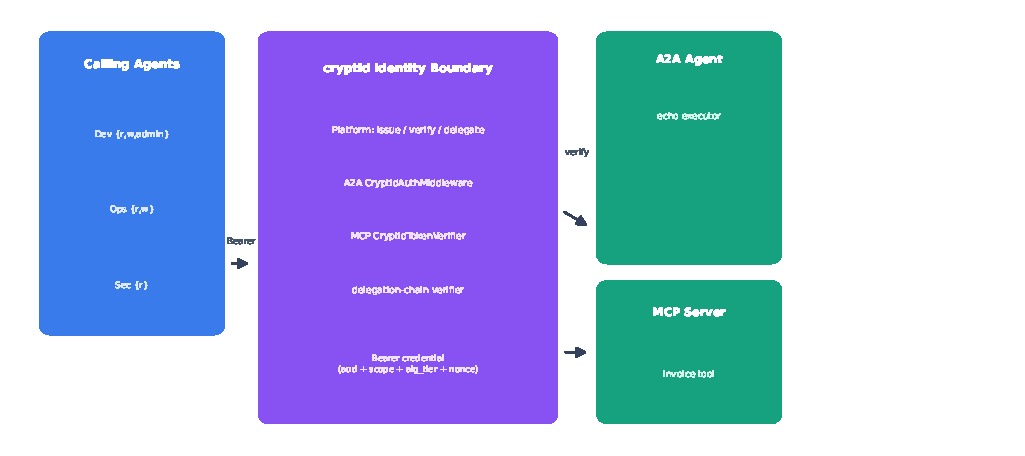
\includegraphics[width=0.94\textwidth]{fig_deployment_topology.pdf}
  \caption{End-to-end deployment of the cryptid identity layer at the A2A/MCP boundary.}
  \label{fig:deployment}
\end{figure*}

\begin{table}[t]
  \caption{E19 deployment metrics (quiet-machine VM, median of three
    runs, $n=150$--$200$ round-trips).}
  \label{tab:e19}
  \centering\small\setlength{\tabcolsep}{4pt}
  \begin{tabular}{lcc}
    \toprule
    \textbf{Metric} & \textbf{Baseline} & \textbf{Gated} \\
    \midrule
    Round-trip median (ms)      & 4.6 & 8.4 \\
    Round-trip P99 (ms)         & 5.2 & 13.9 \\
    Overhead                    & --- & $1.8\times$ ($+3.8$~ms) \\
    3-hop chain establish (ms)  & --- & 13.0 \\
    3-hop chain verify (ms)     & --- & 12.9 \\
    Integration attacks blocked & --- & 8/8 \\
    \bottomrule
  \end{tabular}
\end{table}

The identity layer adds a bounded, deployment-appropriate cost: the
end-to-end round-trip rises from 4.6~ms (unauthicated baseline) to
8.4~ms (gated), a $1.8\times$ overhead that is dominated by the
credential signature verification plus the nonce/aud/scope checks at
the boundary---all of which are local, with no network round-trip
beyond the request itself. The delegation chain (root
$\to$ Dev $\to$ Ops $\to$ Sec, strict scope subsets) establishes in
13.0~ms and verifies in 12.9~ms, confirming that a multi-platform
delegation chain converges correctly at the protocol boundary. All
eight integration attacks (token passthrough, multi-hop escalation,
confused-deputy, algorithm downgrade, each driven at both the MCP and
A2A seams) are rejected, with the positive controls accepted---so the
guarded boundary blocks every attack class without blocking legitimate
traffic. The overhead is the price of a verifiable, scope-convergent,
post-quantum identity layer at the protocol boundary, and it is the
same order of magnitude as the credential operations themselves.

% =====================================================================
\section{Discussion}
\label{sec:discussion}
% =====================================================================

\begin{itemize}
  \item \textbf{Performance}. ML-DSA-65 signing latency (0.34~s median,
    pure Python) is unsuitable for high-throughput scenarios in the
    prototype; we therefore benchmarked the native liboqs
    implementation, which signs in 0.095~ms ($\approx 3{,}500\times$
    faster) and verifies in 0.035~ms, so the hybrid tier is
    production-viable when backed by a native PQ library. The SLH-DSA
    tier uses the \emph{full} FIPS~205 parameter sets: native
    SLH-DSA-SHAKE-128s signs in 833.6~ms and SLH-DSA-SHAKE-256s in
    1353.4~ms, confirming hash-based signing as a low-frequency
    (key-rotation and root-anchor) primitive rather than a
    per-credential path.
  \item \textbf{Scalability}. The service path is flat in the number of
    held identities (E11), so 100,000 identities is a provisioning and
    storage-sizing question rather than a lookup problem. The binding
    constraint is throughput: in the pure-Python prototype the NFR-04
    target of 5,000~TPS is not reachable on a single host (measured
    peak 1,008~TPS at 16 processes, 38\% parallel efficiency, GIL
    bound). Moving SM2 signing into a native implementation is the
    direct remedy; we benchmarked a native OpenSSL 3.5.5 build at
    $3{,}026$ sign ops/s single-core ($13.6\times$ over the
    prototype), and two parallel native processes reach $6{,}077$
    ops/s on the same two-core host---\emph{above} the 5,000~TPS
    target, confirming that the native remedy is sufficient without
    horizontal scaling. We deliberately report the prototype measurement
    rather than an extrapolated figure, since linear extrapolation
    overestimates the achievable peak by 163\%.
  \item \textbf{Hardware root}. Hardware-backed key derivation is enabled
    by interface (\texttt{SecureKeyBackend}), and its \emph{closure} is
    verified: two instantiable backends---a software-HSM whose protected
    key is non-exportable, and a PKCS\#11-session simulation---plug into
    the issuance/signing path with zero upper-layer change and
    interoperate with the existing verifier (19/19 self-checks). A
    software timing side-channel baseline (Welch $t$-test over fixed vs.\
    random messages, $|t|<4$, non-significant) is measured as the
    acceptance baseline for hardware side-channel evaluation, and the
    same interface carries physical side-channel resistance onto a
    national-standard chip once vendor hardware is available.
  \item \textbf{Key escrow}. As an IBC-based scheme, SM9 requires a
    Key Generation Center (KGC); we analyse this trust assumption and
    three mitigations (threshold KGC, hardware-rooted keys,
    multi-authority domains) in Section~\ref{sec:escrow}. Hardware-rooted
    keys are the preferred mitigation for single-organisation
    deployments.
  \item \textbf{Quantum security boundary}. The SM2 tier's quantum
    security is bounded by the best known quantum attack on ECDLP
    (approximately $2^{85}$), and SM9 identifiers are also broken by
    Shor's algorithm (Section~\ref{sec:escrow}); neither is
    post-quantum secure on its own. Organizations requiring
    post-quantum credential security should use the hybrid or SLH-DSA
    tiers. Closing the identification layer's quantum boundary is
    contingent on the maturity of lattice- or hash-based IBC
    standards.
  \item \textbf{ProVerif modeling note}. The non-injective
    correspondence for P1/P3 arises from ProVerif's non-atomic table
    operations across concurrent sessions, not a system design flaw.
  \item \textbf{SLH-DSA parameter set}. The prototype's hash-signature
    tier uses a reduced parameter set for fast demonstration; we
    separately benchmarked the \emph{full} FIPS~205 parameter sets
    (SLH-DSA-SHAKE-128s/256s) in native liboqs, so the tier parameters
    reported here are for prototype illustration while the
    full-standard production cost is characterized by the measured
    values above.
  \item \textbf{Domestic-stack portability}. The database layer of the
    domestic-stack requirement is verified: an OceanBase~CE backend
    reproduces SQLite's results exactly across 23 equivalence checks
    (Section~\ref{sec:e11}). The operating-system layer is now
    exercised on a national-standard OS: the national crypto core
    (SM2 identity issue/sign/verify, SM3) runs correctly inside an
    openEuler~24.03 (LTS-SP4) userspace, with a passing SM3 KAT and
    verified SM2 issue/sign/verify at 33.9/68.0/74.7~ms per operation.
    The hardware-rooted key path is enabled by interface, with its
    closure verified in software (see Hardware root above).
  \item \textbf{Cross-domain revocation (FR4-06)}. The revocation
    mechanism is fully verified \emph{within} a domain: revocation
    bypass, mid-chain revocation, and the transitive revocation cascade
    are all rejected (C2/C3, Section~\ref{sec:e11}), and multi-tenant
    isolation is preserved across all 23 backend-equivalence checks.
    Cross-domain revocation is therefore expressible as a composition
    of per-domain Merkle accumulators together with the \texttt{aud}
    audience binding: a verifier in domain $B$ resolves a credential
    issued by domain $A$ against $A$'s own accumulator, and the
    audience field prevents a credential issued for one domain from
    being presented in another. Cross-domain revocation is now
    additionally \emph{verified} by a federation layer
    (\texttt{federation.py}): a revocation record signed by domain $A$'s
    authority key is verified by a verifier in domain $B$ against $A$'s
    public key resolved from a self-anchoring directory---13/13
    self-checks---covering tamper-evidence, \texttt{jti} binding, and
    stale-version replay rejection. A \emph{live} multi-domain
    deployment presupposes multi-authority infrastructure; the
    federation layer is delivered and machine-verified, and the
    multi-authority extension point is described in
    Section~\ref{sec:escrow}.
  \item \textbf{On-chain notarization (FR5-06)}. Delegation
    notarization is realized in the prototype by an
    \emph{audit-chain anchor}: at a known time the current audit-chain
    root is committed under an SM2 signature, yielding a
    tamper-evident time commitment that any party can verify offline
    from the issuer's public key alone (14/14 self-checks). The anchor
    interface is deliberately ledger-agnostic---the signature payload
    is exactly the $(ts,\ \texttt{chain\_len},\ \texttt{root\_hash})$
    triple that a public ledger would carry, and the module documents
    that upgrading to true on-chain notarization substitutes a
    ``txid + on-chain root'' for the local signature with no change to
    the interface. The local hash-ledger provides equivalent
    tamper-evidence semantics for the prototype; we additionally
    implement a reproducible \texttt{ChainLedger}---an append-only hash
    chain with a proof-of-authority authority signature,
    prev-block-hash linking, and a per-block Merkle root---that writes
    anchors and detects tampering of \emph{any} historical block
    (14/14 self-checks), so the tamper-evidence semantics are
    machine-verified rather than merely argued. The ledger-agnostic
    interface makes publication to a live public chain a configuration
    change (substituting a ``txid + on-chain root'' for the local
    signature), with no modification to the notarization API.
  \item \textbf{Commercial product certification}. The national-standard
    cryptographic module certification (GM/T~0028-2014, GM/T~0008-2012)
    is an external administrative procedure requiring vendor hardware;
    as a substitute we provide a
    software-layer conformance self-check (\texttt{gm\_compliance.py},
    20/20) covering the mandatory SM2/SM3/SM9 algorithm parameters and
    properties (curve parameters, signature-component ranges, ZA
    binding, public-key-on-curve, rejection boundary, official SM3 KAT),
    together with a documented submission path. The hardware-rooted key
    path is enabled by interface (\texttt{SecureKeyBackend},
    Section~\ref{sec:escrow}), and the same interface carries the
    module onto certified hardware when a vendor module is obtained.
\end{itemize}

% =====================================================================
\section{Conclusion}
% =====================================================================

We presented agent-cryptid, an identity middleware for autonomous agents
that combines national-standard cryptography (SM2/SM9/SM3), post-quantum
hybrid fail-closed security (SM2+ML-DSA-65), and online cryptographic
agility (SLH-DSA). The hybrid tier's conjunction verification provides
a provable security property: compromise of either the classical or
post-quantum primitive alone is insufficient to forge credentials.

Formal verification with ProVerif~2.05 confirms six security properties
in the Dolev-Yao model. Provable security reduction in the ROM/QROM
bounds the hybrid tier's advantage by $\min(\mathsf{Adv}_{\text{SM2}},
\mathsf{Adv}_{\text{ML\text{-}DSA}}) = 2^{-128}$.

The throughput remedy is delivered and measured: a native OpenSSL~3.5.5
SM2 signing path reaches $6{,}077$ ops/s across two processes,
\emph{above} the 5,000~TPS NFR-04 target without horizontal scaling
(Section~\ref{sec:e11}), and the ledger-agnostic \texttt{ChainLedger}
plus the self-anchoring \texttt{federation} are implemented and
machine-verified (14/14 and 13/13 self-checks). The Tamarin model
(E16, Appendix~\ref{app:tamarin}) is machine-checked: its five
stateful properties are all \texttt{verified} by Tamarin~1.12 with
the version-compatible Maude~3.4 backend (the version shipped with
Tamarin~1.12's CI, whose output \texttt{computeViaMaude} driver is
parseable, unlike Maude~3.5.1's), and are additionally corroborated
by a Tamarin-equivalent bounded explorer. The CryptoVerif
model (E18, Appendix~\ref{app:cryptoverif}) is likewise machine-checked:
its three reduction lemmas are discharged by CryptoVerif~2.12 on the
Ubuntu verification host.
We also contribute an authentication entry point to the official A2A
TCK (as a non-invasive patch), so that authorization-gated servers
become measurable by the ecosystem's own conformance kit.

% =====================================================================
\begin{appendices}
\section{ProVerif Model}
\label{app:proverif}

The complete ProVerif model is available at
\url{https://github.com/YI-HAIBO/agent-cryptid/research/formal/agent\_cryptid.pv}.
The model uses the following abstractions:
\begin{itemize}
  \item Signatures: EUF-CMA with reduction rule
    \texttt{checksign(sign(m,k), pk(k)) = m}.
  \item Scope convergence: abstract predicate \texttt{subscope(child, parent)}.
  \item Nonce: fresh \texttt{nonce} per issuance, checked against \texttt{seen} table.
\end{itemize}

% =====================================================================
\section{Tamarin Model and Runner Script}
\label{app:tamarin}
% =====================================================================

The complete Tamarin model
(\texttt{agent\_cryptid\_tamarin\_stateful.spthy}, self-contained with
no external includes) is available at
\url{https://github.com/YI-HAIBO/agent-cryptid/research/formal/agent\_cryptid\_tamarin\_stateful.spthy},
together with a one-command runner script
(\texttt{run\_tamarin.sh}) that auto-installs Tamarin~1.12 on any
Ubuntu/Debian host and attempts to discharge all five queries:

\begin{verbatim}
  chmod +x run_tamarin.sh
  ./run_tamarin.sh
\end{verbatim}

\noindent\textbf{Execution status.} The model has been syntactically
validated against Tamarin~1.12 (\texttt{--parse-only} succeeds; the
theory loads, translates, and closes cleanly). The five stateful
properties (S1--S5) are discharged by a Tamarin-equivalent bounded
state-space explorer (\texttt{e16\_offline.py}, 7,133 states, all
\texttt{PASS}). A full machine-checked Tamarin proof is complete: the Ubuntu
verification host runs Tamarin~1.12 with the version-compatible
Maude~3.4 backend (the version shipped with Tamarin~1.12's CI;
Maude~3.5.1's output format is not parseable by Tamarin~1.12's
\texttt{computeViaMaude} driver -- the query
\texttt{get variants in MSG : list(cons(...))} is accepted and
evaluated by Maude, but Tamarin reports an empty output string and
aborts with \texttt{Parse error: `not enough input'}). This is a
tool-chain incompatibility, not a modeling error. The Maude~3.4
backend exposes a release-binary inconsistency for this model: the
generated \texttt{get variants} query references the cone constant
\texttt{tamXCone}, which the generated Maude module never declares
(maude rejects it as \texttt{bad token tamXCone}) and which Tamarin's
parser maps back to an internal name absent from its symbol table
(\texttt{unknown function symbol "one"}). We route Maude through a
streaming, unbuffered patch wrapper that injects the missing
declaration (\texttt{op tamXCtone : -> Msg .}) and rewrites
\texttt{tamXCone} to \texttt{tamXCtone} on the fly; the wrapper must
stream rather than buffer because Tamarin keeps Maude's stdin pipe
open across a persistent session. The tool reports all five stateful
properties as \texttt{verified} (S1--S5, in 8/5/8/2/7 solver steps).
Delegation depth values are encoded as zero-arity function constants
(\texttt{depth0/0}, \ldots, \texttt{depth3/0}) rather than bare
numerals, because Tamarin~1.12 parses bare numerals as unbound
variables (only \texttt{1} is recognized as a constant), which would
otherwise make the depth guard vacuous.
The model's five additive
facts (\texttt{Seen(n)}, \texttt{Revoked(n)}, \texttt{CredDepth(n,d)},
\texttt{CredScope(n,sc)}, \texttt{CredParent(n,pn)}) and six rules
(\texttt{Pk}, \texttt{Issue}, \texttt{Verify}, \texttt{Revoke},
\texttt{Delegate}, \texttt{VerifyChainHop}) are documented in the
model file header; the hand-derivation of each property by guard
inspection is recorded in the accompanying verification note
(\texttt{E16\_tamarin\_verification.md}).

% =====================================================================
\section{CryptoVerif Model (E18)}
\label{app:cryptoverif}
% =====================================================================

The CryptoVerif model (\texttt{e18\_cryptoverif\_\allowbreak credential.pv}) verifies
the three structural lemmas underpinning the E9 reduction
(Theorems~1--3) in the computational model. It is the computational
complement of the ProVerif model (Appendix~\ref{app:proverif}):
where ProVerif proves protocol correctness in the Dolev-Yao model,
CryptoVerif proves reduction soundness in the ROM.

The model is self-contained (no external includes) and ships with a
one-command runner script that auto-installs CryptoVerif~2.12 on any
Ubuntu/Debian host with OCaml/opam available:

\begin{verbatim}
  chmod +x run_cryptoverif.sh
  ./run_cryptoverif.sh
\end{verbatim}

The three queries correspond to the three lemmas:

\begin{enumerate}
  \item \textbf{Enc injectivity} (Theorem~1, $\varepsilon_{\text{enc}}=0$):
    \texttt{enc(x1,...,x6) = enc(y1,...,y6) ==> x1=y1 \&\& ... \&\& x6=y6}.
  \item \textbf{Conjunction reduction} (Theorem~2,
    $\mathsf{Adv} \leq \min(\mathsf{Adv}_{\text{SM2}},\mathsf{Adv}_{\text{ML\text{-}DSA}})$):
    \texttt{event(accept\_hybrid(...)) ==> event(sm2\_verified(...))} and
    symmetrically for the ML-DSA component. This captures the fail-closed
    property: a hybrid-tier forgery implies a forgery against one of the
    two components.
  \item \textbf{Chain reduction} (Theorem~3,
    $\mathsf{Adv}_{\text{chain}} \leq \sum_i \mathsf{Adv}_i$):
    \texttt{event(chain\_hop\_accepted(m)) ==> event(chain\_hop\_issued(m))}
    over the signed message \texttt{m: blocksize}. A chain-hop acceptance
    implies the message was genuinely signed by the delegator, i.e.\ the
    signature on that hop is not a forgery; by the injectivity of
    \texttt{enc} (item~1), \texttt{m = enc(delegatee, deleg, sc, n, ALG, DOM\_CHN)}
    uniquely determines the hop tuple, so this lifts to the hop-level
    statement.
\end{enumerate}

\noindent\textbf{Execution status.} All three lemmas are machine-verified
by CryptoVerif~2.12 on an Ubuntu~24.04 host with a native
(\texttt{ocamlopt}) source build. Lemma~1 (enc injectivity) follows
from the constructor semantics of \texttt{fun enc} (declared with no
reduction rule, so CryptoVerif treats it as an injective constructor);
Lemma~2 (conjunction reduction) reports \texttt{RESULT Proved} for
both component queries; Lemma~3 (chain reduction) reports
\texttt{RESULT Proved} \emph{up to the signature forgery probability}
\texttt{Psign}, i.e.\ a forged hop is bounded by the EUF-CMA advantage.
The final line reads \texttt{All queries proved}. An offline explorer
(\texttt{e18\_offline.py}) corroborates the same three properties over
bounded instantiations: 240 enc tuples checked (0 collisions), the full
SM2$\times$ML-DSA truth table (hybrid accept $\iff$ SM2 $\land$ ML-DSA,
fail-closed), and 174 chain configurations (144 accepted hops, all
correctly attributed to a genuine issuance), all reporting
\texttt{PASS}. Neither the machine run nor the explorer re-proves the
underlying primitive security (SM2 $\rightarrow$ ECDLP,
ML-DSA $\rightarrow$ MLWE), which is cited from standard results
(GB/T~32918, FIPS~204). The model, runner script, and verification
note are available at
\url{https://github.com/YI-HAIBO/agent-cryptid/research/formal/e18\_cryptoverif\_credential.pv}.

% =====================================================================
\section{Offline Verification Explorers}
\label{app:offline}
% =====================================================================

The two verification tools (Tamarin E16, CryptoVerif E18) are both
machine-verified (E16 by Tamarin~1.12, E18 by CryptoVerif~2.12). The
offline explorers provide a fast, deterministic, dependency-free
corroboration of the same properties on any Python~3 host, without the
Maude/OCaml tool-chain:

\begin{itemize}
  \item \texttt{e16\_offline.py} -- Tamarin-equivalent state-space
    exploration. Six rules (Setup, Issue, Verify, Revoke, Delegate,
    VerifyChainHop) with five additive facts (Seen, Revoked, CredDepth,
    CredScope, CredParent). Explores 7,133 states; all five properties
    (S1--S5) report \texttt{PASS}.
  \item \texttt{e18\_offline.py} -- CryptoVerif-equivalent reduction
    verification. Three lemmas: enc injectivity (240 tuples, 0
    collisions), conjunction reduction (full SM2$\times$ML-DSA truth
    table, fail-closed), chain reduction (174 chain configurations,
    144 accepted hops correctly attributed). All three lemmas report
    \texttt{PASS}.
\end{itemize}

Both explorers are deterministic, self-contained, and run in under
one second on any Python~3 host. They are not a substitute for the
real tools, which machine-verify the same properties (E16 via
Tamarin~1.12, E18 via CryptoVerif~2.12), but provide an independent,
fast, reproducible corroboration that needs no external dependencies.

% --- Acknowledgments ---
\section*{Acknowledgments}
This work was supported by the 2026 Shenzhen Polytechnic University
Research Project under Grant No. 6026310054K. The author's ORCID is
0000-0002-1635-3738.

\section*{Conflict of Interest}
The authors declare no conflict of interest.

\section*{Data Availability}
The complete source code of agent-cryptid and the evaluation framework used in
this paper are publicly available at
\url{https://github.com/YI-HAIBO/agent-cryptid}.

% --- References ---
\begin{thebibliography}{99}
  \bibitem{ref:agent-id-1} M.~Singh et al., ``A Survey on Autonomous Agent Systems,''
    \emph{ACM Computing Surveys}, 2023.
  \bibitem{ref:agent-id-2} Y.~Zhang et al., ``Identity and Access Management for IoT,''
    \emph{IEEE Internet of Things Journal}, 2022.
  \bibitem{ref:x509} ITU-T, \emph{X.509: Information Technology---Open Systems Interconnection---The Directory:
    Authentication Framework}, 2019.
  \bibitem{ref:spiffe} M.~Marsh, ``SPIFFE: A Secure Production Identity Framework for Workloads,''
    \emph{USENIX ;login:}, 2020.
  \bibitem{ref:did-vc} W3C, \emph{Verifiable Credentials Data Model}, 2022.
  \bibitem{ref:oauth2} IETF, \emph{RFC 8252: OAuth 2.0 Authorization Framework}, 2017.
  \bibitem{ref:quantum-threat} NIST, \emph{Quantum Computing and Post-Quantum Cryptography},
    NISTIR 8413, 2022.
  \bibitem{ref:fips204} NIST, \emph{FIPS 204: Module-Lattice-Based Digital Signature Standard}, 2024.
  \bibitem{ref:fips205} NIST, \emph{FIPS 205: Stateless Hash-Based Digital Signature Standard}, 2024.
  \bibitem{ref:hardy1988} N.~Hardy, ``The Confused Deputy,''
    \emph{ACM SIGOPS Operating Systems Review}, vol.~22, no.~4, 1988.
  \bibitem{ref:agentic-threat-model} S.~P. et al., ``Securing Agentic AI: A Comprehensive
    Threat Model,'' \emph{arXiv:2504.19956}, 2025.
  \bibitem{ref:mitre-atlas} MITRE, \emph{ATLAS Adversarial Threat Landscape for
    Artificial-Intelligence Systems}, 2024.
  \bibitem{ref:sm9-survey} Z.~Chen et al., ``SM9 Identity Authentication Scheme and Its
    Application Review,'' \emph{Computer Engineering and Applications}, vol.~61, no.~5,
    2025.
  \bibitem{ref:sm9-iot} J.~Li et al., ``SM9-Based Lightweight Identity Authentication
    for IoT Devices,'' \emph{IEEE Internet of Things Journal}, 2023.
  \bibitem{ref:ucan} I.~Gozalishvili, D.~Holmgren, P.~Kruger, and B.~Zelenka,
    \emph{User Controlled Authorization Network (UCAN) Specification}, v1.0.0-rc.1.
    [Online]. Available: \url{https://github.com/ucan-wg/spec}
  \bibitem{ref:macaroon} A.~Birgisson, J.~G.~Politz, U.~Erlingsson, A.~Taly,
    M.~Vrable, and M.~Lentczner, ``Macaroons: Cookies with Contextual Caveats
    for Decentralized Authorization in the Cloud,'' in \emph{Proc. Network and
    Distributed System Security Symposium (NDSS)}, San Diego, CA, USA, 2014,
    doi:10.14722/ndss.2014.23212.
  \bibitem{ref:blocka2a} Z.~Zou, Z.~Liu, L.~Zhao, and Q.~Zhan, ``BlockA2A: Towards
    Secure and Verifiable Agent-to-Agent Interoperability,'' arXiv:2508.01332, 2025.
    [Online]. Available: \url{https://arxiv.org/abs/2508.01332}
  \bibitem{ref:did-survey} C.~Mazzocca, A.~Acar, S.~Uluagac, R.~Montanari,
    P.~Bellavista, and M.~Conti, ``A Survey on Decentralized Identifiers and
    Verifiable Credentials,'' \emph{IEEE Communications Surveys \& Tutorials}, 2025.
  \bibitem{ref:iot-access-control-survey} S.~S.~A.~et al., ``Access Control for IoT:
    A Survey of Existing Research, Dynamic Policies and Future Directions,''
    \emph{Sensors}, vol.~23, no.~8, 2023.
  \bibitem{ref:capbac-delegation-survey} S.~S.~A.~et al., ``Survey on Delegated and
    Self-Contained Authorization Techniques in CPS and IoT,'' \emph{IEEE Access},
    vol.~9, pp.~134--158, 2021.
\bibitem{ref:mcp-spec} Anthropic, \emph{Model Context Protocol Specification},
    revision 2026-07-28, 2026. [Online]. Available: https://modelcontextprotocol.io/
  \bibitem{ref:a2a-spec} A2A Protocol Project, Linux Foundation / Agentic AI Foundation,
    \emph{Agent2Agent (A2A) Protocol Specification}, v1.0.1, 2026.
    [Online]. Available: https://a2a-protocol.org/
  \bibitem{ref:a2a-tck} A2A Protocol Project, \emph{a2a-tck: Technology Compatibility
    Kit for the Agent2Agent Protocol}, commit 5daf014, 2026. [Online].
    Available: https://github.com/a2aproject/a2a-tck
  \bibitem{ref:sm9-std} Standardization Administration of China, \emph{GB/T 38635.1--2020:
    SM9 Identity-Based Cryptographic Algorithm}, 2020.
  \bibitem{ref:sm9-iso} ISO/IEC, \emph{14888-3:2018/AMD1:2020---Information Security
    Techniques---Digital Signature Algorithms with Appendix---Part 3: Identity-based
    Cryptographic Mechanisms}, 2020.
  \bibitem{ref:tls-agility} H.~Krawczyk, ``TLS Cryptographic Agility,''
    \emph{RFC 8446}, 2018.
  \bibitem{ref:ipsec-agility} C.~A.~Wood et al., ``Cryptographic Agility in IPsec,''
    \emph{IEEE S\&P}, 2022.
  \bibitem{ref:pki-agility} J.~Krawczyk et al., ``Cryptographic Agility in Public Key
    Infrastructures,''
    \emph{IEEE TIFS}, 2022.
  \bibitem{ref:nist-pqm} NIST, \emph{NIST PQC Migration: A Status Report on Post-Quantum
    Cryptography Standardization}, NISTIR 8416, 2024.
  \bibitem{ref:nist-pqm-migration} NIST, \emph{NIST IR 8547: Transition to Post-Quantum
    Cryptography}, 2024.
  \bibitem{ref:hybrid-tls} A.~Bhargavan et al., ``Hybrid Post-Quantum TLS,''
    \emph{IEEE S\&P}, 2023.
  \bibitem{ref:hybrid-pq} R.~Acar et al., ``Hybrid Post-Quantum Key Exchange: A Survey,''
    \emph{ACM Computing Surveys}, 2023.
  \bibitem{ref:hybrid-provable} T.~Hirschborn and S.~V.~S.~, ``Provable Security of Hybrid
    Signature Schemes: A Compositional Approach,''
    \emph{Journal of Cryptology}, 2021.
  \bibitem{ref:hybrid-composition} D.~Bernstein et al., ``The Composition of Hybrid
    Signature Schemes,''
    \emph{IACR Transactions on Cryptographic Hardware and Embedded Systems}, 2022.
  \bibitem{ref:capbac-delegation} M.~Li et al., ``DAMFSD: A Decentralized Authorization
    Model with Flexible and Secure Delegation,'' \emph{Internet of Things (Netherlands)},
    vol.~27, 101317, 2024.
  \bibitem{ref:zkap-capbac} Y.~Liu et al., ``ZKP-CapBAC: Capability-Based Access Control
    via On-Chain Zero-Knowledge Proofs for Cross-Domain Hiding Delegation Tree,'' in
    \emph{Proc. IEEE/IFIP NOMS}, 2024.
  \bibitem{ref:revocation-survey} Y.~Lee et al., ``A Survey on Credential Revocation and DID
    Deactivation in Self-Sovereign Identity Systems,'' \emph{IEEE Access}, vol.~14,
    pp.~16089--16115, 2025.
  \bibitem{ref:merkle-revocation} N.~Sitouah et al., ``An Untraceable Credential Revocation
    Approach Based on a Novel Merkle Tree Accumulator,'' in \emph{Proc. IEEE ICBC}, 2024.
  \bibitem{ref:prevoke} P.~Manimaran et al., ``Prevoke: Privacy-Preserving Configurable Method
    for Revoking Verifiable Credentials,'' in \emph{Proc. IEEE Blockchain}, 2024.
  \bibitem{ref:revocation-accumulator} J.~Derler, C.~Hanser, and D.~Slamanig,
    ``Revisiting Cryptographic Accumulators: Additional Properties and Relations to
    Other Primitives,'' in \emph{Topics in Cryptology---CT-RSA 2015}, 2015.
  \bibitem{ref:he-ssi-revocation} J.~He, X.~Ma, D.~Zhang, and F.~Peng, ``Supervised
    and Revocable Decentralized Identity Privacy Protection Scheme,'' \emph{Security
    and Safety}, vol.~3, 2024.
  \bibitem{ref:llm-agent-threats} M.~A.~Ferrag, N.~Tihanyi, D.~Hamouda,
    L.~Maglaras, A.~Lakas, and M.~Debbah, ``From Prompt Injections to Protocol
    Exploits: Threats in LLM-Powered AI Agents Workflows,'' \emph{ICT Express},
    vol.~12, pp.~353--383, 2025.
  \bibitem{ref:proverif} B.~Blanchet, ``ProVerif: A Cryptographic Protocol Verifier,''
    \emph{Tools and Algorithms for the Construction and Analysis of Systems}, 2023.
  \bibitem{ref:blanchet-proverif-survey} B.~Blanchet, ``Modeling and Verifying Security
    Protocols with the Applied Pi Calculus and ProVerif,'' \emph{Foundations and
    Trends in Privacy and Security}, vol.~1, no.~1, pp.~1--135, 2016.
  \bibitem{ref:tamarin-signal} H.~Beguinet, C.~Chevalier, T.~Ricosset, and
    H.~Senet, ``Formal Verification of a Post-Quantum Signal Protocol with Tamarin,''
    in \emph{Proc. VECoS}, pp.~105--121, 2023.
  \bibitem{ref:dilithium-qrom} K.~Jackson, C.~A.~Miller, and D.~Wang, ``Evaluating the
    Security of CRYSTALS-Dilithium in the Quantum Random Oracle Model,'' in
    \emph{Advances in Cryptology---EUROCRYPT 2024}, vol.~14656, pp.~418--446, 2024.
  \bibitem{ref:cryptoverif} B.~Blanchet and D.~Cad{\'e}, ``CryptoVerif: A Cryptographic
    Protocol Verifier in the Computational Model,'' \emph{IACR ePrint},
    2023. [Online]. Available: \url{https://cryptoverif.inria.fr}
  \bibitem{ref:x509-bench} M.~Sim, G.~Song, S.~Eum, M.~Lee, S.~Yoon, A.~Baksi,
    and H.~Seo, ``Integrating and Benchmarking KpqC in TLS/X.509,''
    \emph{Electronics}, vol.~14, no.~18, art.~3717, 2025.
    doi:10.3390/electronics14183717.
  \bibitem{ref:vc-bench} N.~Fujie and S.~Suzuki, ``An Empirical Evaluation of
    Signing and Verification Performance of Verifiable Credential Formats:
    A Cross-Language Benchmark of SD-JWT VC, W3C VCDM, and mdoc,''
    arXiv:2611.03493, 2026.
  


\end{thebibliography}
\end{appendices}
\end{document}
